\documentclass[english]{article}
\usepackage[a4paper, total={6in, 9in}]{geometry}
\usepackage[utf8]{inputenc}
\usepackage{listings}
\usepackage{color}
\usepackage[dvipsnames, table]{xcolor}
\usepackage{graphicx}
\usepackage[T1]{fontenc}
\usepackage{babel}
\usepackage{caption}
\usepackage{subcaption}
\usepackage[title]{appendix}
\usepackage{float}
\usepackage{attachfile}
\usepackage[
backend=biber,
style=numeric,
sorting=ynt
]{biblatex}

% makes the figure counting be on a section by section basis
\counterwithin{figure}{section}
\counterwithin{table}{section}

\addbibresource{base.bib}

\title{Simulating Aircraft Boarding Strategies\\
\large DAT530 project}

\author{
Rihab Al Zurkani\\
Faculty of Science and Technology\\
University of Stavanger
\and
Stephan Frederik Werner Brandasu\\
Faculty of Science and Technology\\
University of Stavanger
}

\date{November 2022}



\definecolor{codegreen}{rgb}{0,0.6,0}
\definecolor{codegray}{rgb}{0.5,0.5,0.5}
\definecolor{codepurple}{rgb}{0.58,0,0.82}
\definecolor{backcolour}{rgb}{0.95,0.95,0.92}
% sets the codeblock style
\lstset{
    language=MATLAB,
    backgroundcolor=\color{backcolour},   
    commentstyle=\color{codegreen},
    keywordstyle=\color{magenta},
    numberstyle=\tiny\color{codegray},
    stringstyle=\color{codepurple},
    basicstyle=\ttfamily\footnotesize,
    columns=fullflexible,
    frame=single,
    breaklines=true,
    postbreak=\mbox{\textcolor{red}{$\hookrightarrow$}\space},
    numbers=left,
    stepnumber=1,
    showstringspaces=false,
    tabsize=1,
    breakatwhitespace=false,
}


\begin{document}

\maketitle
\pagenumbering{gobble}
\newpage

\pagenumbering{roman}
\tableofcontents
\newpage

\begin{abstract}
    We describe 3 methods of boarding an airplane modeled in $GPenSIM$. The models will take advantage of pre and post processors to delay transitions to simulate queues inside the aircraft and use coloured tokens to assign tokens to specific places in the plane.
\end{abstract}
\newpage



\pagenumbering{arabic}
\section{Introduction}
% Problem Definition
\subsection{Problem Statement}
In this project we will model 3 different methods of how passengers could potentially board a plane. 2 of these models will be based off of the design and results from \citetitle{STEFFEN201264} by \citeauthor{STEFFEN201264}\cite{STEFFEN201264}. The last model will be a combination of the 2 other models to see if that would improve them or not.

This is an important process to model because as they say 'time is money', and neither the passengers nor the airline wants to waste unnecessary time when boarding the plane.


\subsection{Challenges}
There are 2 primary challenges when modeling the system. These challenges are the 'aisle block' and the 'seat shuffle'. We will describe scenarios for these challenges with table \ref{tab:example_plane} as a visual guide for both cases.

\begin{table}[H]
    \centering
    \begin{tabular}{|c|c|c|c|c|c|c|}
    \hline
    \rowcolor{lightgray}\multicolumn{7}{|c|}{front}\\
    \hline
        1A & 1B & 1C & \cellcolor{lightgray} & 1D & 1E & 1F \\
        2A & 2B & 2C & \cellcolor{lightgray} & 2D & 2E & 2F \\
        3A & 3B & 3C & \cellcolor{lightgray} & 3D & 3E & 3F \\
        4A & 4B & 4C & \cellcolor{lightgray} & 4D & 4E & 4F \\
        5A & 5B & 5C & \cellcolor{lightgray} & 5D & 5E & 5F \\
        6A & 6B & 6C & \cellcolor{lightgray} & 6D & 6E & 6F \\
    \hline
    \end{tabular}
    \caption{First 6 rows of an aircraft, people enter the plane from the front}
    \label{tab:example_plane}
\end{table}

In the case of the aisle block what could happen is that your seat is in \emph{5B}, but the person who entered the plane in front of you is sitting in \emph{4B}. In this situation, you have to wait for the person in front of you to sit down before you can progress to your own seat. This is obviously an inefficiency in terms of time. But for the model to replicate this something needs to be put in place to stop a person from progressing while somebody else in front of them is sitting down.

Meanwhile for the seat shuffle say that you're entering the plane and your seat is \emph{5A}, but somebody is already sitting in \emph{5B}. In this situation, the person in \emph{5B} needs to get up, go back into the aisle, you can then go to your seat, and then they can go back into their seat. This will substantially increase the time it takes to sit down and again relating to the previously mentioned problem, it will increase the aisle waiting time too. Unfortunately, this one will likely be impossible to properly model due to $GPenSIM$' lack of variable firing time support. 


\section{Method \& Design}
% overall design, approach, techniques, alternatives

\subsection{Boarding Strategies}
As mentioned previously we will attempt to model 3 different boarding strategies in \emph{GPenSIM}. 2 of these would come from \citetitle{STEFFEN201264} and they can be seen in table \ref{tab:paper_methods}. 

Table \ref{tab:wilma_group} shows the Wilma model. The advantage of this model is that you completely avoid the seat shuffle scenario. Since the boarding groups are based on the column you sit within the people sitting on the ends of the rows always board first, while the people sitting in the aisle seats board last.

Table \ref{tab:block_group} shows the Block model. The advantage of this model is that the chance of serious aisle blocking where your seat is further back in the plane but you have to wait for somebody who sits closer to the front is massively reduced. This model doesn't do anything to address the seat shuffle though.

\begin{table}[H]
    \begin{subtable}[h]{0.45\textwidth}
        \centering
        \begin{tabular}{|c|c|c|c|c|c|c|}
        \hline
        \rowcolor{lightgray}\multicolumn{7}{|c|}{front}\\
        \hline
        1 & 2 & 3 & \cellcolor{lightgray} & 3 & 2 & 1 \\
        1 & 2 & 3 & \cellcolor{lightgray} & 3 & 2 & 1 \\
        1 & 2 & 3 & \cellcolor{lightgray} & 3 & 2 & 1 \\
        1 & 2 & 3 & \cellcolor{lightgray} & 3 & 2 & 1 \\
        1 & 2 & 3 & \cellcolor{lightgray} & 3 & 2 & 1 \\
        1 & 2 & 3 & \cellcolor{lightgray} & 3 & 2 & 1 \\
        1 & 2 & 3 & \cellcolor{lightgray} & 3 & 2 & 1 \\
        1 & 2 & 3 & \cellcolor{lightgray} & 3 & 2 & 1 \\
        1 & 2 & 3 & \cellcolor{lightgray} & 3 & 2 & 1 \\
        1 & 2 & 3 & \cellcolor{lightgray} & 3 & 2 & 1 \\
        1 & 2 & 3 & \cellcolor{lightgray} & 3 & 2 & 1 \\
        1 & 2 & 3 & \cellcolor{lightgray} & 3 & 2 & 1 \\
        \hline
        \end{tabular}
       \caption{Wilma boarding groups}
       \label{tab:wilma_group}
    \end{subtable}
    \hfill
    \begin{subtable}[h]{0.45\textwidth}
        \centering
        \begin{tabular}{|c c c|c|c c c|}
    \hline
    \rowcolor{lightgray}\multicolumn{7}{|c|}{front}\\
    \hline
        2 & 2 & 2 & \cellcolor{lightgray} & 2 & 2 & 2 \\
        2 & 2 & 2 & \cellcolor{lightgray} & 2 & 2 & 2 \\
        2 & 2 & 2 & \cellcolor{lightgray} & 2 & 2 & 2 \\
        2 & 2 & 2 & \cellcolor{lightgray} & 2 & 2 & 2 \\
        \hline
        3 & 3 & 3 & \cellcolor{lightgray} & 3 & 3 & 3 \\
        3 & 3 & 3 & \cellcolor{lightgray} & 3 & 3 & 3 \\
        3 & 3 & 3 & \cellcolor{lightgray} & 3 & 3 & 3 \\
        3 & 3 & 3 & \cellcolor{lightgray} & 3 & 3 & 3 \\
        \hline
        1 & 1 & 1 & \cellcolor{lightgray} & 1 & 1 & 1 \\
        1 & 1 & 1 & \cellcolor{lightgray} & 1 & 1 & 1 \\
        1 & 1 & 1 & \cellcolor{lightgray} & 1 & 1 & 1 \\
        1 & 1 & 1 & \cellcolor{lightgray} & 1 & 1 & 1 \\
    \hline
    \end{tabular}
        \caption{Block boarding groups}
        \label{tab:block_group}
     \end{subtable}
     \caption{Different boarding models from\citetitle{STEFFEN201264}\cite{STEFFEN201264} }
     \label{tab:paper_methods}
\end{table}

As an attempt to combine the advantages of both models we want to try a combined Wilma-Block model which can be seen in table \ref{tab:wilmablock_group}. In theory, this model should combine the advantage of Wilma where the seat shuffle should never happen, and the advantage of the Block model where aisle blocking should happen less often.  

\begin{table}[H]
    \centering
        \begin{tabular}{|c|c|c|c|c|c|c|}
    \hline
    \rowcolor{lightgray}\multicolumn{7}{|c|}{front}\\
    \hline
        4 & 5 & 6 & \cellcolor{lightgray} & 6 & 5 & 4 \\
        4 & 5 & 6 & \cellcolor{lightgray} & 6 & 5 & 4 \\
        4 & 5 & 6 & \cellcolor{lightgray} & 6 & 5 & 4 \\
        4 & 5 & 6 & \cellcolor{lightgray} & 6 & 5 & 4 \\
        \hline
        7 & 8 & 9 & \cellcolor{lightgray} & 9 & 8 & 7 \\
        7 & 8 & 9 & \cellcolor{lightgray} & 9 & 8 & 7 \\
        7 & 8 & 9 & \cellcolor{lightgray} & 9 & 8 & 7 \\
        7 & 8 & 9 & \cellcolor{lightgray} & 9 & 8 & 7 \\
        \hline
        1 & 2 & 3 & \cellcolor{lightgray} & 3 & 2 & 1 \\
        1 & 2 & 3 & \cellcolor{lightgray} & 3 & 2 & 1 \\
        1 & 2 & 3 & \cellcolor{lightgray} & 3 & 2 & 1 \\
        1 & 2 & 3 & \cellcolor{lightgray} & 3 & 2 & 1 \\
    \hline
    \end{tabular}
    \caption{Wilma-Block combined method}
    \label{tab:wilmablock_group}
\end{table}

Those advantages are only in theory though. It should also be considered that this model is more for curiosity than it is a practical alternative. At some point, boarding groups become too small and there's just no way people are going to line up in groups this small when waiting to enter a plane.


\subsection{The Model}
The model will be described in 2 pieces, first the airplane and then the gate to enter the airplane.

\subsubsection{The Aircraft}
The aircraft as seen in figure \ref{fig:plane} is made up of a series of places that are connected by a single transition between them. Each place along the plane represents the space in the aisle of an airplane along the rows of seats. 

\begin{figure}[H]
    \centering
    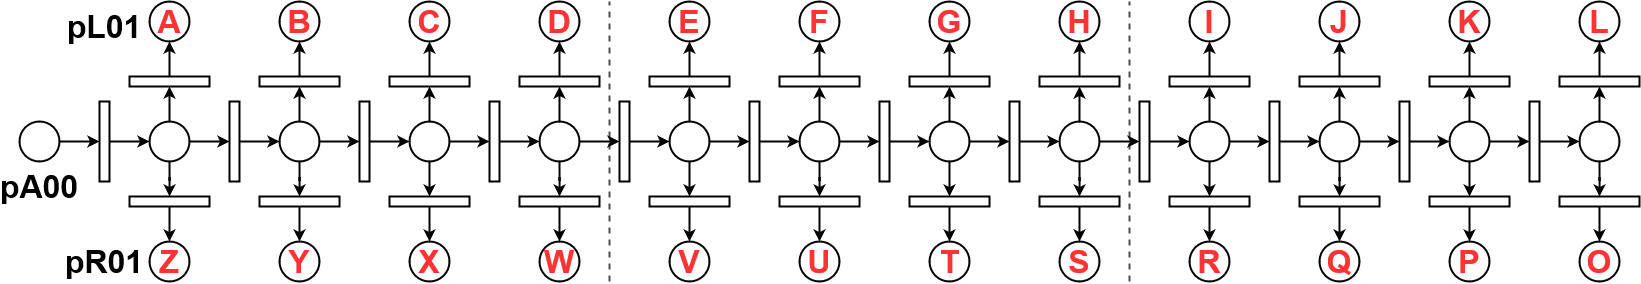
\includegraphics[width=\textwidth]{figures/plane.jpg}
    \caption{Basic overview of the aircraft model}
    \label{fig:plane}
\end{figure}

The individual rows of seats are treated as a single place in our model. This is because of GPenSIM' lack of variable firing time support which means that the seat shuffle cannot be simulated. The transitions feeding the tokens from the aisle into the given row do so by looking for a token with a specific colour. On the left side of the airplane, each row goes up through the alphabet while the right side goes down through the alphabet. This was simply done for clarity while developing and to more quickly visually distinguish where a token needs to go when troubleshooting strange behavior. 

The transition between each of the aisle places will disable itself after firing. This is to prevent an aisle place from ever holding more than a single token thereby simulating when passengers start being backed up in the plane. To illustrate how this works we should look at figure \ref{fig:plane_zoom} which is a zoomed version of what is shown in figure \ref{fig:plane}.

\begin{figure}[H]
    \centering
    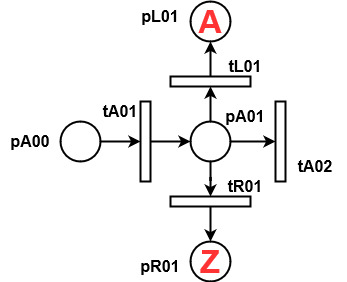
\includegraphics[width=0.4\textwidth]{figures/plane zoom.jpg}
    \caption{Zoomed in view of start of plane}
    \label{fig:plane_zoom}
\end{figure}

When a token passes through \lstinline{Ta01} it will disable itself. From there while the token sits in \lstinline{pA01} it will be grabbed by one of the available transitions, The side transitions \lstinline{tL01} and \lstinline{tR01} have an increased priority to make sure that if the correct coloured token exists in \lstinline{pA01} it will always be grabbed by the correct side transition. If the token doesn't match the required colour for the side transitions it will continue forward in \lstinline{tA02}. Any one of \lstinline{tL01}, \lstinline{tR01} or \lstinline{tA02} will re-enable \lstinline{tA01} in their post-processor. It is placed in the post-processor to simulate the wait from if somebody is sitting down in their seat. We don't want other tokens to progress through the aisle until the side transition has finished firing.

To deal with the lack of variable firing time support the firing time of the side transitions are simply increased or decreased depending on if the current model being tested has a chance of the seat shuffle occurring or not. 

The name for the places and transitions are a short description of their location. So the aisle places are \lstinline{pA00}-\lstinline{pA12} for example, the full naming scheme can be seen in the following list:

\begin{itemize}
    \item Aisle places: \lstinline{pA00}-\lstinline{pA12}
    \item Aisle Transitions: \lstinline{tA01}-\lstinline{tA12}
    \item Left places: \lstinline{pL01}-\lstinline{pL12}
    \item Left transitions: \lstinline{tL01}-\lstinline{tL12}
    \item Right places: \lstinline{pR01}-\lstinline{pR12}
    \item Right transitions: \lstinline{tR01}-\lstinline{tR12}
\end{itemize}

The numbering will always line up with each other so all the places numbered '1' will always be in line with each other and the transitions numbered '1' will always feed into places that are also numbered '1'. This can be seen in figure \ref{fig:plane_zoom}.

The airplane model does not change depending on which boarding strategy is being tested. But when a strategy which involves boarding groups made up of groups of rows is being tested then the rows get effectively get divided as shown by the dotted lines in figure \ref{fig:plane}.

\subsubsection{The Gate}
The 'gate' is where the uncoloured tokens start from, get turned into coloured tokens and continue to the rest of the plane. There are 2 different variations of the gate depending on how the passengers are being grouped on entry. There is either a single transition which colours all the tokens which would be named \lstinline{tInit} as shown in figure \ref{fig:basic_init} or there are multiple transitions that effectively split the tokens into groups, as shown in figure \ref{fig:group_init}.

\begin{figure}[H]
    \centering
    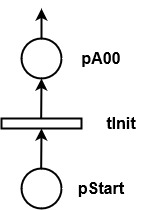
\includegraphics[height=5cm]{figures/basic_init.jpg}
    \caption{Single group initialise}
    \label{fig:basic_init}
\end{figure}

With the single \lstinline{tInit} tokens will simply pass through the transition and get a colour. This colour is decided by cycling over a list of every possible colour 3 times. every colour comes up 3 times to accurately simulate the situation where maybe there's a family sitting next to each other. They won't board separately from each other regardless of the current strategy so this is included with the colour selection. To make the colour rotation random on every run the list of colours gets shuffled when running the simulation.

The \lstinline{tInit} transition has the same behaviour as the aisle transitions mentioned previously where it will disable itself after firing. Same as before this is to avoid any place after \lstinline{pStart} to ever hold more than 1 token at the time (excluding the seats).

\begin{figure}[H]
    \centering
    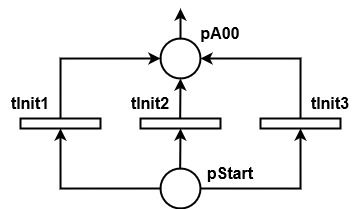
\includegraphics[width=8cm]{figures/group_init.jpg}
    \caption{row by row group based boarding initialise}
    \label{fig:group_init}
\end{figure}

In the strategy where the boarding groups are made up of rows we replace the single \lstinline{tInit} with 3 of them; \lstinline{tInit1}, \lstinline{tInit2} and \lstinline{tInit3}. Here each transition can only give colours belonging to its boarding group. Meaning that \lstinline{tInit1} with the block boarding previously described will only be able to give the colours that are behind the 2nd dotted line in figure \ref{fig:plane}. 

To prevent the groups from mixing with each other these transitions just like before will fire only 1 at a time to avoid multiple tokens existing in the aisle places simultaneously. They also have another check which is to see which boarding group is current active. If that variable is set to '1' then only \lstinline{tInit1} can fire, if its set to '2' then only \lstinline{tInit2} can fire. To transition from 1 group to another the transitions will count how many times they've fired. Once they've fired 24 times they will disable themselves and allow the next transition to fire. Having it like this should make sure that 1 group will always finish entering the plane before the next one can start.


\subsection{Design Alternative}
Instead of using pre and post processors to block the aisle transitions from firing it would be possible to use a new place connected to each of the transitions for a given row as shown in figure \ref{fig:aisle_block_alt}.

\begin{figure}[H]
    \centering
    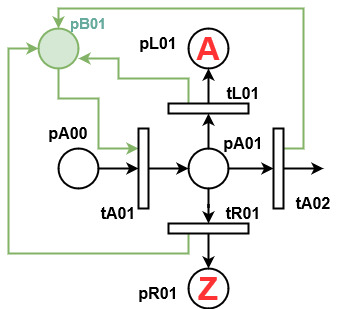
\includegraphics[width=0.5\textwidth]{figures/aircraft-zoom-alt.jpg}
    \caption{Alternate method of blocking aisle, the new arcs and place are shown in green.}
    \label{fig:aisle_block_alt}
\end{figure}

This new place would effectively do the same thing as the current pre and post processor solution because when \lstinline{tA01} fires it would take the token from \lstinline{pB01}, when this token is taken \lstinline{tA01} can no longer fire until either \lstinline{tL01}, \lstinline{tR01} or \lstinline{tA02} returns the token back to \lstinline{pB01}. 

The reason we didn't do it this way is because the model already has a large number of places and arcs. Adding a bunch of extra arcs and places would open the door to make a mistake when defining the Petri Net much more than the current solution. Additionally it would bloat the Petri Net Definition file so much that finding a mistake would quickly become a nightmare. So it was decided that the easiest way to approach the problem was with common pre and post processors. 


\section{Implementation}
% coding of components
\subsection{Main}
\subsubsection{Colour Rotation}
Regardless of which model is being made the main file looks relatively similar. It will start with setting the colour rotation which the \lstinline{tInit} transitions use to draw colours from, this will get randomly shuffled and saved into a global variable together with the current index of the list. This can be seen in figure \ref{fig:colour_list}.

\begin{figure}[H]
    \centering
\begin{lstlisting}[language=MATLAB]
% full list of coloured tokens
colourRotation = {'A','B','C','D','E','F','G','H','I','J','K','L' ...
    'A','B','C','D','E','F','G','H','I','J','K','L' ...
    'A','B','C','D','E','F','G','H','I','J','K','L' ...
    'Z','Y','X','W','V','U','T','S','R','Q','P','O' ...
    'Z','Y','X','W','V','U','T','S','R','Q','P','O' ...
    'Z','Y','X','W','V','U','T','S','R','Q','P','O'};

% set the colour rotation to be random
global_info.cr = colourRotation(randperm(numel(colourRotation)));

% colour rotation index
global_info.cr_index = 0;
\end{lstlisting}
    \caption{The list of all possible colours from the Wilma model that get shuffled and saved}
    \label{fig:colour_list}
\end{figure}

In the case of the block boarding models each group has its own separate colour rotation which gets individually created, shuffled and saved as shown in figure \ref{fig:colour_listblock}.

\begin{figure}[H]
    \centering
\begin{lstlisting}[language=MATLAB]
% full list of coloured tokens
colourRotation2 = {'A','B','C','D' ...
    'A','B','C','D' ...
    'A','B','C','D' ...
    'Z','Y','X','W' ...
    'Z','Y','X','W' ...
    'Z','Y','X','W'};
colourRotation3 = {'E','F','G','H' ...
    'E','F','G','H' ...
    'E','F','G','H' ...
    'V','U','T','S' ... 
    'V','U','T','S' ...
    'V','U','T','S'};
colourRotation1 = {'I','J','K','L' ...
    'I','J','K','L' ...
    'I','J','K','L' ...
    'R','Q','P','O' ...
    'R','Q','P','O' ...
    'R','Q','P','O'};

% set the colour rotation to be random
global_info.cr1 = colourRotation1(randperm(numel(colourRotation1)));
global_info.cr2 = colourRotation2(randperm(numel(colourRotation2)));
global_info.cr3 = colourRotation3(randperm(numel(colourRotation3)));
\end{lstlisting}
    \caption{The list of all possible colours split up for the Block model that get shuffled and saved}
    \label{fig:colour_listblock}
\end{figure}


\subsubsection{Aisle Blocking}
From there every single blockable transition has its global blocking variable defined, all of them defaulting to open in this case. Additionally as shown on line $1$ and $2$ in figure \ref{fig:tblock} the current boarding group and the amount of boarded passengers from the current group is defined. It should be noted that this is not present in the Wilma model but only in the Block boarding group models. This is because these variables are necessary to make the triple initialize transitions shown in figure \ref{fig:group_init} work. But they don't have any purpose in the Wilma model single \lstinline{tInit}.

\begin{figure}[H]
    \centering
\begin{lstlisting}[language=MATLAB]
global_info.boarded = 0;
global_info.currentGroup = 1;

% block the init(s)
global_info.init = 1;
% the aisle blocking variables (1=open, 0=blocked)
global_info.A01 = 1;
global_info.A02 = 1;
global_info.A03 = 1;
global_info.A04 = 1;
global_info.A05 = 1;
global_info.A06 = 1;
global_info.A07 = 1;
global_info.A08 = 1;
global_info.A09 = 1;
global_info.A10 = 1;
global_info.A11 = 1;
global_info.A12 = 1;
\end{lstlisting}
    \caption{All transition blocking variables and the initialize blockers}
    \label{fig:tblock}
\end{figure}


\subsubsection{Firing Times \& Priority}
The firing times were tuned to as best as possible match the results from \citetitle{STEFFEN201264}\cite{STEFFEN201264}. We used \emph{0.5} for the aisle transitions in all models. We treated the firing time of \emph{1} as one second, so with the aisle transition firing time mentioned earlier, that means we estimated that it takes about half a second to walk through each row of the airplane. 

The side transition firing times as mentioned previously were variable depending on which model was being simulated. For the block model since there is a chance of the seat shuffle occurring we used a firing time of \emph{10.5}. In the Wilma model, we used a firing time of \emph{7} because the seat shuffle should be impossible there.

\begin{figure}[H]
    \centering
\begin{lstlisting}[language=MATLAB]
% firing times, Have been tweaked to attempt to closely match the pre-existing results
% from the paper by Jason Steffen and Jon Hotchkiss
dyn.ft = {'tL01',7,'tL02',7,'tL03',7,'tL04',7,'tL05',7,'tL06',7, ...
    'tL07',7,'tL08',7,'tL09',7,'tL10',7,'tL11',7,'tL12',7, ...
    'tR01',7,'tR02',7,'tR03',7,'tR04',7,'tR05',7,'tR06',7, ...
    'tR07',7,'tR08',7,'tR09',7,'tR10',7,'tR11',7,'tR12',7, ...
    'allothers', 0.5};
% transition priority, prioritise side ones to make sure colours go down
% their pathway
dyn.ip = {'tL01',1,'tL02',1,'tL03',1,'tL04',1,'tL05',1,'tL06',1, ...
    'tL07',1,'tL08',1,'tL09',1,'tL10',1,'tL11',1,'tL12',1, ...
    'tR01',1,'tR02',1,'tR03',1,'tR04',1,'tR05',1,'tR06',1, ...
    'tR07',1,'tR08',1,'tR09',1,'tR10',1,'tR11',1,'tR12',1
};
\end{lstlisting}
    \caption{Firing times and transition priority in the Wilma model}
    \label{fig:ft_ip}
\end{figure}

Additionally, the side transitions all had to have their priority increased from the default to make sure that they would always be able to grab their respective coloured token. Without priority, the tokens would frequently go down the aisle and get stuck at the end of the plane.

\subsection{Preprocessor}
\subsubsection{Common Preprocessor}
The common preprocessor would handle the firing conditions for the main aisle and seat transitions. The firing conditions for the \lstinline{tInit}(s) were kept in separate specific preprocessor files. 

The common preprocessor simply checked each aisle transition and would only let it fire if the respective variable was enabled or not, the code in figure \ref{fig:commonpre} has been truncated due to it being unnecessary to show every single transition since they're all almost the same.

\begin{figure}[H]
    \centering
\begin{lstlisting}[language=MATLAB]
if strcmp(trans.name, 'tA01')
    fire = eq(global_info.A01, 1);
elseif strcmp(trans.name, 'tA02')
    fire = eq(global_info.A02, 1);
[...]
elseif strcmp(trans.name, 'tA12')
    fire = eq(global_info.A12, 1);
    
% all the left side transitions, They dont need to disable the aisle
% because it disables it self to be re-enabled for the next token either by
% the left-right transition or by the next aisle transition
elseif strcmp(trans.name, 'tL01')
    tokID1 = tokenEXColor('pA01',1,'A');
    fire = tokID1;
[...]
elseif strcmp(trans.name, 'tR12')
    tokID1 = tokenEXColor('pA12',1,'O');
    fire = tokID1;
else
    fire = 1;
    % nothing special
\end{lstlisting}
    \caption{Truncated view of the transition and aisle firing preprocessor}
    \label{fig:commonpre}
\end{figure}

The side transitions would grab the colour of the token and compare it to what it expects to get, if it is the correct colour it will grab the token and fire thanks to the firing priority mentioned previously. Or if it isn't the correct colour it simply does nothing.

\subsubsection{tInit Preprocessor}
The initialising transition has 2 different preprocessors depending on if the model has block boarding or not. 

In the Wilma boarding case where there is only a single \lstinline{tInit} we can see what the preprocessor looks like in figure \ref{fig:tinit_pre_wilma}. It will simply check if the transition is enabled, if it is then it grabs the index of the color, increments the index, and sets the new colour for the transition. Otherwise, it doesn't fire. It was important to put the color rotation inside of the \lstinline{if} statement because otherwise even when the transition is being blocked it would rotate to the next colour, skipping the current one which we don't want.

\begin{figure}[H]
    \centering
\begin{lstlisting}[language=MATLAB]
if global_info.init == 1
    % give colours to tokens passing through tinit
    index = mod(global_info.cr_index, 72)+1;
    global_info.cr_index = global_info.cr_index + 1;
    transition.new_color = global_info.cr(index);
    fire = 1;
 else
    fire = 0;
end
\end{lstlisting}
    \caption{Wilma model \lstinline{tInit_pre.m}}
    \label{fig:tinit_pre_wilma}
\end{figure}

In the block boarding cases an extra check needs to be added to the \lstinline{if} statement. This check is to make sure that we are currently in the correct group for the transition. For each numbered transition this check is different so in the preprocessor file for \lstinline{tInit2} the \lstinline{if global_info.currentGroup} will want to be equal to \emph{2} instead of \emph{1} as can be seen in figure \ref{fig:tinit_pre_block}

\begin{figure}[H]
    \centering
\begin{lstlisting}[language=MATLAB]
if global_info.currentGroup == 1 && global_info.init == 1
    index = mod(global_info.cr_index, 24)+1;
    global_info.cr_index = global_info.cr_index + 1;
    transition.new_color = global_info.cr1(index);
    fire = 1;
    global_info.boarded = global_info.boarded + 1;
    if global_info.boarded >= 24
       global_info.init = 0;
       global_info.cr_index = 0;
       global_info.boarded = 0;
       global_info.currentGroup = 2;  
    end
else
    fire = 0;
end
\end{lstlisting}
    \caption{Block model \lstinline{tInit1_pre.m}}
    \label{fig:tinit_pre_block}
\end{figure}

The preprocessor will also count the number of tokens it has let through in this case. Once it has let 24 tokens through it has finished its group so it resets the color index, and the boarded count and allows the next group to start boarding. Additionally, it will disable the initialise transitions here because if it doesn't then the other initialise will fire too early meaning that \lstinline{pA00} will have more than 1 token which we don't want.


\subsection{Post Processor}
The post processor is what makes the aisle transitions disable themselves and also re-enable the previous aisle transition. First, all the side transitions will re-enable their own aisle transition, this is to make sure that the aisle transition does start working again. It was placed in the post processor instead of the preprocessor to simulate firing times. We don't want the aisle to continue until after the side has finished firing. 

\begin{figure}[H]
    \centering
\begin{lstlisting}[language=MATLAB]
% re-enable the aisle transition after the side transition has finished firing. 
if strcmp(trans.name, 'tL01')
    global_info.A01 = 1;
elseif strcmp(trans.name, 'tR01')
    global_info.A01 = 1;
[...]
elseif strcmp(trans.name, 'tR12')
    global_info.A12 = 1;
% Aisle transition self disable
elseif strcmp(trans.name, 'tA01')
    global_info.A01 = 0;
    global_info.init = 1;
elseif strcmp(trans.name, 'tA02')
    global_info.A02 = 0;
    global_info.A01 = 1;
[...]
elseif strcmp(trans.name, 'tInit')
    global_info.init = 0;
else
    % nothing
end
\end{lstlisting}
    \caption{Truncated view of \lstinline{COMMON_POST.m}}
    \label{fig:commonpost}
\end{figure}

Further down in the truncated post processor seen in figure \ref{fig:commonpost} we can see the post processor for all the aisle transitions, here they will disable themselves and then re-enable the previous transition in case of a token which is simply just advancing forward to their seat. 





\section{Testing, Analysis \& Results}
% Simple user manual, sample run, describe data used, analysis, originality of this work
\subsection{Verifying That It Works As Intended}
To verify that all the mechanisms of the model work as intended we will plot some of the places in the model over the course of a run to see if we're getting the expected behaviour. 

\subsubsection{Aisle Blocking}
First to verify that the aisle blocking works as intended we will plot each of the aisle places. If an aisle place ever holds more than a single token then the aisle blocking is not working as intended.

\begin{figure}[H]
    \centering
    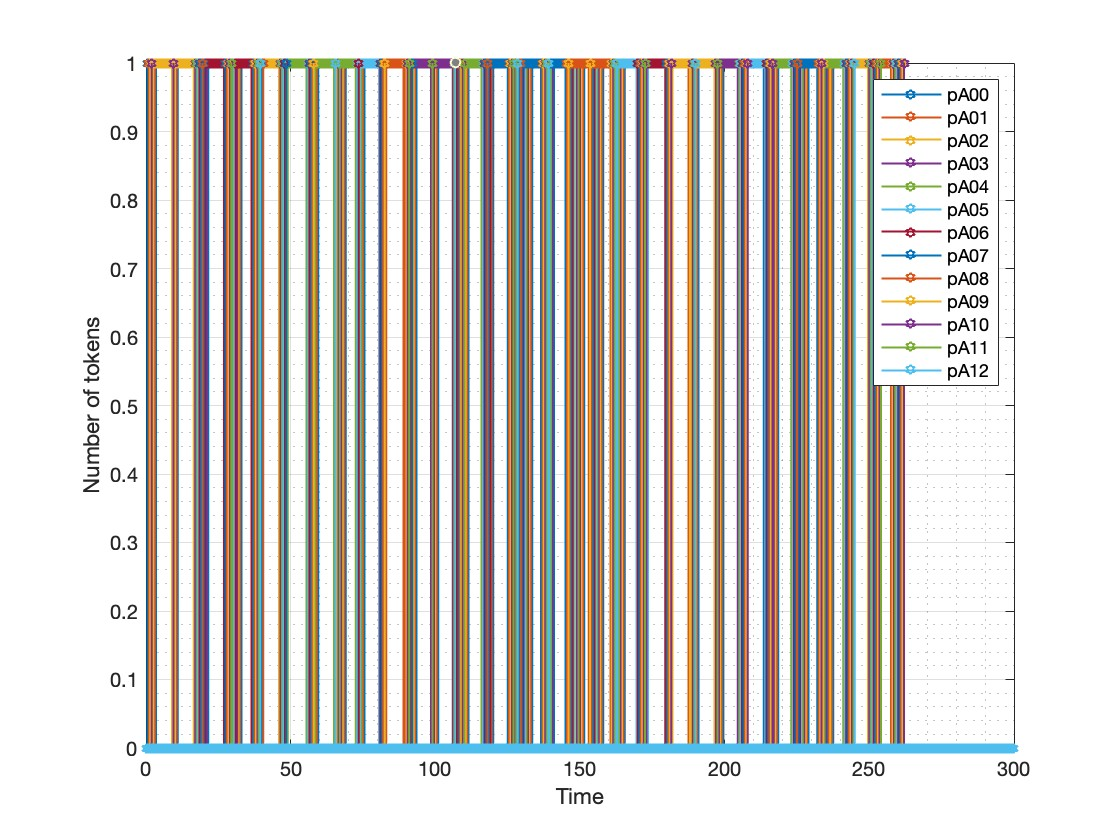
\includegraphics[width=0.6\textwidth]{figures/aisleblockcheck.jpg}
    \caption{Aisle place results after running Wilma model}
    \label{fig:aisle_block_check}
\end{figure}

When we look at figure \ref{fig:aisle_block_check} we can see that at no point does any of the aisle places have more than 1 token at once. This means that the aisle blocking is working as intended.

\subsubsection{Group Boarding}
To make sure that the groups are being boarded in the correct order we will separately plot each group to make sure that they're happening after each other and not getting mixed up. If one group is boarding at the same time as another then the groups are not working as intended. 

\begin{figure}[H]
     \centering
     \begin{subfigure}[b]{0.3\textwidth}
         \centering
         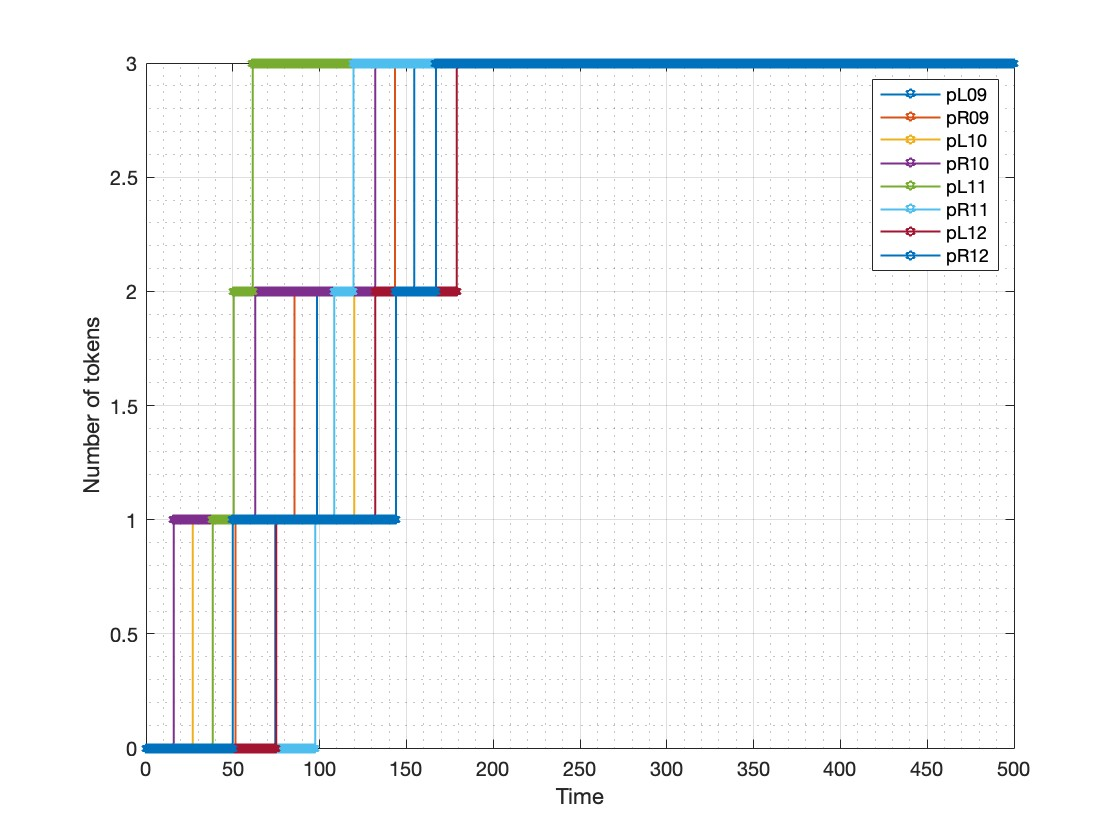
\includegraphics[width=\textwidth]{figures/group1.jpg}
         \caption{group 1}
         \label{fig:group1}
     \end{subfigure}
     \hfill
     \begin{subfigure}[b]{0.3\textwidth}
         \centering
         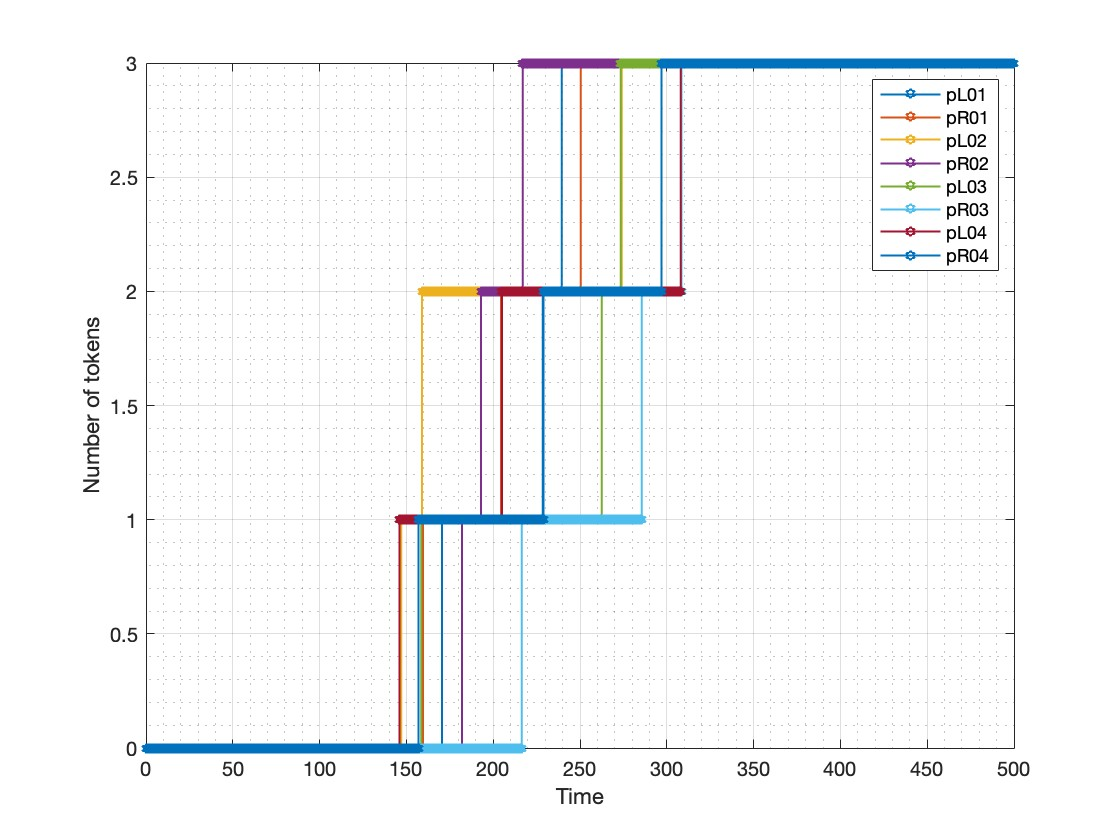
\includegraphics[width=\textwidth]{figures/group2.jpg}
         \caption{group 2}
         \label{fig:group2}
     \end{subfigure}
     \hfill
     \begin{subfigure}[b]{0.3\textwidth}
         \centering
         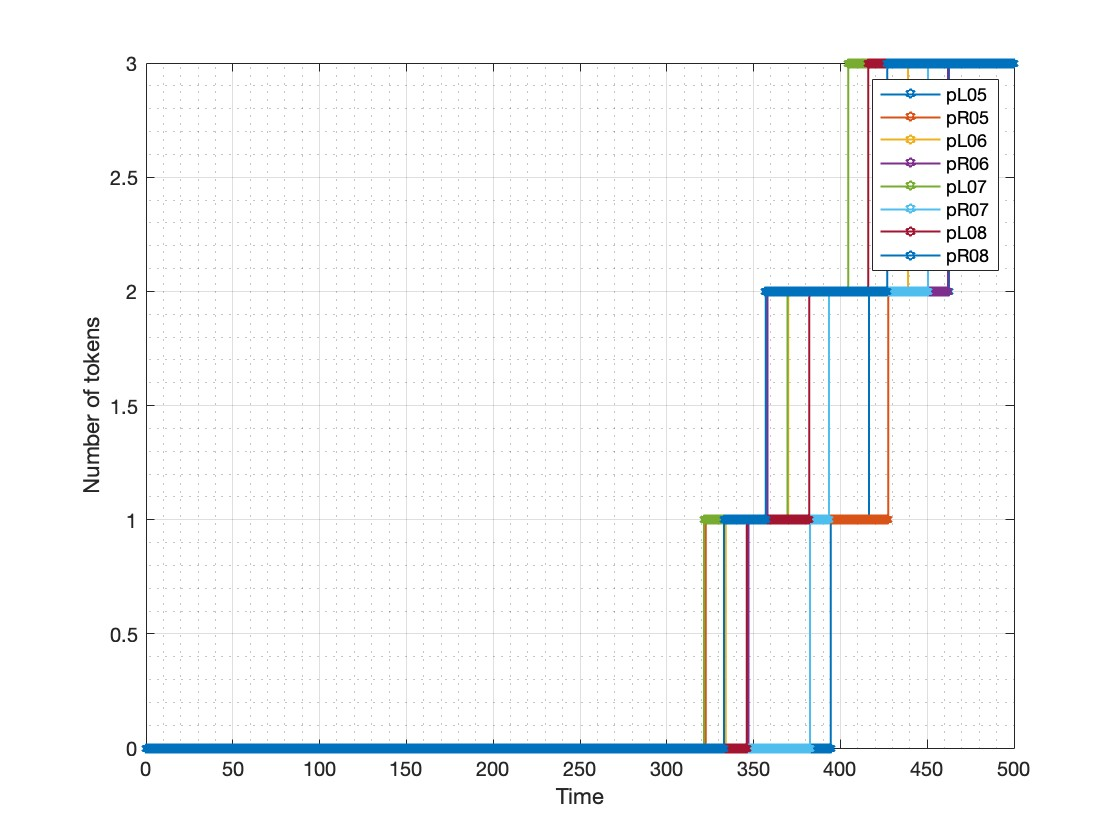
\includegraphics[width=\textwidth]{figures/group3.jpg}
         \caption{group 3}
         \label{fig:group3}
     \end{subfigure}
        \caption{The 3 boarding groups in the block model}
        \label{fig:groupboarding}
\end{figure}

We can see in figure \ref{fig:groupboarding} that each group happens one after the other exactly like they should so the group boarding is also working exactly as intended. 

\subsubsection{Correct Seating Positions}
To check if all tokens are getting to their seat we look at the output of \lstinline{prnss(sim)}. Every side transition should have 3 tokens in it at the end, and no tokens should exist anywhere else in the model. 

\begin{figure}[H]
    \centering
    \begin{lstlisting}[language=MATLAB]
**    Time: 462.5   **
State: 612
Fired Transition: tL05
Current State: 3pL01 + 3pL02 + 3pL03 + 3pL04 + 3pL05 + 3pL06 + 3pL07 + 3pL08 + 3pL09 + 3pL10 + 3pL11 + 3pL12 + 3pR01 + 3pR02 + 3pR03 + 3pR04 + 3pR05 + 3pR06 + 3pR07 + 3pR08 + 3pR09 + 3pR10 + 3pR11 + 3pR12   
Virtual tokens: (no tokens)
\end{lstlisting}
    \caption{Block model prnss output}
    \label{fig:blockprnss}
\end{figure}

In figure \ref{fig:blockprnss} we can see that every side place has 3 tokens at the end of the simulation so that is working as intended.

\begin{figure}[H]
    \centering
    \begin{lstlisting}[language=MATLAB]
**    Time: 258.5   **
State: 612
Fired Transition: tL10
Current State: 3pL01 + 3pL02 + 3pL03 + 3pL04 + 3pL05 + 3pL06 + 3pL07 + 3pL08 + 3pL09 + 3pL10 + 3pL11 + 3pL12 + 3pR01 + 3pR02 + 3pR03 + 3pR04 + 3pR05 + 3pR06 + 3pR07 + 3pR08 + 3pR09 + 3pR10 + 3pR11 + 3pR12   
Virtual tokens: (no tokens)
\end{lstlisting}
    \caption{Wilma model prnss output}
    \label{fig:wilmaprnss}
\end{figure}

Similarly as before for the Wilma model we can also see in figure \ref{fig:wilmaprnss} that every place ends up with 3 tokens so every token is clearly making it to the correct place.

\subsection{Output \& Firing Times}
When we run the main simulation files we get a few different outputs, first of all in the console the state of the tokens gets printed as shown in figure \ref{fig:blockprnss} and \ref{fig:wilmaprnss}. 

Additionally it will make multiple figures. The first one is as shown in figure \ref{fig:aisle_block_check} used to verify that the aisle block is working as intended for that given run. Additionally it will print out a figure which shows how the seats filled up over the entire time of the model and for the block boarding method it will print a figure for each individual block as shown in figure \ref{fig:groupboarding}.

As mentioned the plots only exist for verification. The main interest we have is to see the final time of the model because that's what tells us how long it took to finish boarding the plane. For figure \ref{fig:wilmaprnss} we can see that this specific run of the Wilma model took 258.5 seconds. In figure \ref{fig:blockprnss} we can see that this specific run of the Block model took 462.5 seconds.

All the firing times were set partially by imagining how long things takes and partially by trial and error to as closely as possible replicate the results from \citetitle{STEFFEN201264}\cite{STEFFEN201264}.

These firing times should be relatively accurate to how long it would take in real life since they're based on real experimentation and it is relatively easily to just test your self how long it takes to walk a short distance or how long it takes to sit down. 


\subsection{Results}
Each aircraft boarding model was run 10 times, we will compare the averages to see how they stack up against each other in table \ref{tab:results_all}.

\begin{table}[H]
    \centering
\begin{tabular}{|c|c|c|c|}
    \hline
    Model & Target & Tested Average & Tested Standard Deviation \\
    \hline
    Wilma & 253 & 253.15 & 15.35\\
    \hline
    Block & 414 & 425.2 & 13.07 \\
    \hline
    WilmaBlock & <253 & 303.72 & 12.06 \\
    \hline
\end{tabular}
    \caption{Simulation results for each model}
    \label{tab:results_all}
\end{table}

Here it is important to remember that the times from the Wilma and the Block model were designed to come as close as possible to the results from \citetitle{STEFFEN201264}\cite{STEFFEN201264}. The goal of these models was to replicate their results as a baseline for our firing times, not to create our own strategy. 

Meanwhile unfortunately in the model we did make ourselves, which is a combination of the Wilma model and the Block model the result is somehow worse than one of the Wilma models on its own. This would seem strange except \citetitle{STEFFEN201264} also has similar results. They found that letting passengers in at random, so everybody enters at once in one big group performs better than the Block model. It seems there is some inefficiency to letting people enter this sort of back-to-front group so the fastest realistically achievable method would be the Wilma method. 

Interestingly though it seems that the standard deviation goes down with the block-based methods. This won't offset how much overall slower they are. But it does mean they give more consistent overall results.


\section{Discussion}
\subsection{Results Discussion}
We have successfully modeled 2 of the boarding strategies from \citetitle{STEFFEN201264} and created our own hybrid in \emph{GPenSIM}. While the result of our hybrid strategy isn't what we hoped for it isn't entirely unexpected considering that \citetitle{STEFFEN201264} also has some unexpected results where somehow having less specific boarding groups gives better results.

What we still achieved with our models of the Wilma and the Block method is that now that this exists in $GPenSIM$ it could relatively easily be expanded to see how each method scales when you increase the size of the plane. 

Additionally running the simulation is almost instant compared to testing this with actual people so having this modeled in $GPenSIM$ allows us to test how big the variance of results is within a given model or maybe see if a certain result is an outlier. 

\subsection{Limitations}
It would have been nice if there was a way to simulate the seat shuffle. The only way we thought of implementing it would be to have a variable firing time based on chance. There should be a $\frac{2}{3}$ chance of the seat shuffle occurring so having that be the chance of a slower fire would allow for the model to have a lot more depth. 

There might be a more 'hacky' solution to the seat shuffle but it would likely be a nightmare to implement on a larger scale. 

Additionally we are not certain whether the result of the Wilma-Block combined method is correct or not. Despite the fact that the original paper showed some models being surprisingly bad, where they were worse than letting everybody board at random. It feels like there could be a chance that something with how the transitions are disabling themselves and then being re-enabled might be inefficient which causes some issues for the block-based models that shouldn't be there. 

Doing more runs of each model to get a larger and more accurate dataset is also something that is missing in our work. To make that sustainable over a large number of attempts (100+) it would require some method of automating starting the run and logging the results.

\subsection{Future Work}
Given more time it would be possible to expand the models we have built into the same scale as full-size aircraft and also model all the different models suggested in \citetitle{STEFFEN201264}. 

The model could also be expanded to simulate 2-aisle wide-body airplanes but this would require testing to find realistic firing times and would substantially complicate the logic for how tokens travel down the aisle to get to their row. 

\subsection{Learning Experiences}
Getting the transition to disable to work as intended was surprisingly difficult and as mentioned before we're still not sure if it's fully working how we want. Once that fell into a relatively good working state though everything was surprisingly intuitive and straightforward from there. 

What was especially positive was how we could use the common pre and post processor separately from the specific ones used for the initialization transitions. This meant we could have all the 'basic' on-off switches in 1 bigger file while keeping slightly more advanced logic in individual files.




\newpage
\printbibliography


\begin{appendices}


\section{Installation guide}
No additional libraries are needed, make sure when adding the models to path that only 1 is added at the time of running. If multiple models are in the path at the same time then it causes strange unintended behaviour in the results.

\section{User Manual}
The simulation files can be found in the $simulation$ directory with a different subdirectory for each simulated model. To run a model enter the subdirectory for the desired model and simply run the file named after the model $.m$. So for the Wilma model you go to $simulation/wilma/wilma.m$ and run it.

\section{Complete Code - ZIP}
The link below contains a zip file with all the simulation files in separate directories named after which model it is. Each directory also contains a README file with a table showing each individual result, the average and the target from \citetitle{STEFFEN201264}.
\\
\\
\textattachfile{simulation.7z}{\textcolor{blue}{simulation.7z}}

\section{Complete Code}

\subsection{Wilma}
\begin{lstlisting}[language=MATLAB, caption=COMMON\_POST.m]
function [] = COMMON_POST(trans)

global global_info

% re-enable the aisle transition after the side transition has finished
% firing. 
if strcmp(trans.name, 'tL01')
    global_info.A01 = 1;
elseif strcmp(trans.name, 'tR01')
    global_info.A01 = 1;
elseif strcmp(trans.name, 'tL02')
    global_info.A02 = 1;
elseif strcmp(trans.name, 'tR02')
    global_info.A02 = 1;
elseif strcmp(trans.name, 'tL03')
    global_info.A03 = 1;
elseif strcmp(trans.name, 'tR03')
    global_info.A03 = 1;
elseif strcmp(trans.name, 'tL04')
    global_info.A04 = 1;
elseif strcmp(trans.name, 'tR04')
    global_info.A04 = 1;
elseif strcmp(trans.name, 'tL05')
    global_info.A05 = 1;
elseif strcmp(trans.name, 'tR05')
    global_info.A05 = 1;
elseif strcmp(trans.name, 'tL06')
    global_info.A06 = 1;
elseif strcmp(trans.name, 'tR06')
    global_info.A06 = 1;
elseif strcmp(trans.name, 'tL07')
    global_info.A07 = 1;
elseif strcmp(trans.name, 'tR07')
    global_info.A07 = 1;
elseif strcmp(trans.name, 'tL08')
    global_info.A08 = 1;
elseif strcmp(trans.name, 'tR08')
    global_info.A08 = 1;
elseif strcmp(trans.name, 'tL09')
    global_info.A09 = 1;
elseif strcmp(trans.name, 'tR09')
    global_info.A09 = 1;
elseif strcmp(trans.name, 'tL10')
    global_info.A10 = 1;
elseif strcmp(trans.name, 'tR10')
    global_info.A10 = 1;
elseif strcmp(trans.name, 'tL11')
    global_info.A11 = 1;
elseif strcmp(trans.name, 'tR11')
    global_info.A11 = 1;
elseif strcmp(trans.name, 'tL12')
    global_info.A12 = 1;
elseif strcmp(trans.name, 'tR12')
    global_info.A12 = 1;
% when the aisle transitions fire they should disable themselves to prevent
% a single aisle place from having more than 2 tokens at once. a aisle
% transition can then re-enable the previous aisle transition to avoid it
% being blocked forever.
elseif strcmp(trans.name, 'tA01')
    global_info.A01 = 0;
    global_info.init = 1;
elseif strcmp(trans.name, 'tA02')
    global_info.A02 = 0;
    global_info.A01 = 1;
elseif strcmp(trans.name, 'tA03')
    global_info.A03 = 0;
    global_info.A02 = 1;
elseif strcmp(trans.name, 'tA04')
    global_info.A04 = 0;
    global_info.A03 = 1;
elseif strcmp(trans.name, 'tA05')
    global_info.A05 = 0;
    global_info.A04 = 1;
elseif strcmp(trans.name, 'tA06')
    global_info.A06 = 0;
    global_info.A05 = 1;
elseif strcmp(trans.name, 'tA07')
    global_info.A07 = 0;
    global_info.A06 = 1;
elseif strcmp(trans.name, 'tA08')
    global_info.A08 = 0;
    global_info.A07 = 1;
elseif strcmp(trans.name, 'tA09')
    global_info.A09 = 0;
    global_info.A08 = 1;
elseif strcmp(trans.name, 'tA10')
    global_info.A10 = 0;
    global_info.A09 = 1;
elseif strcmp(trans.name, 'tA11')
    global_info.A11 = 0;
    global_info.A10 = 1;
elseif strcmp(trans.name, 'tA12')
    global_info.A12 = 0;
    global_info.A11 = 1;
elseif strcmp(trans.name, 'tInit')
    global_info.init = 0;
else
    % nothing
end
\end{lstlisting}



\begin{lstlisting}[language=MATLAB, caption=COMMON\_PRE.m]
% COMMON_PRE.m
function [fire, trans] = COMMON_PRE(trans)
global global_info

tokID1 = [];

% first we handle the aisle, the logic here is that the aisle can only fire
% when its been enabled. The aisle will get disabled while the side
% transitions are firing to simulate people blocking the aisle while they
% stow their baggage and move into their seat.
if strcmp(trans.name, 'tA01')
    fire = eq(global_info.A01, 1);
elseif strcmp(trans.name, 'tA02')
    fire = eq(global_info.A02, 1);
elseif strcmp(trans.name, 'tA03')
    fire = eq(global_info.A03, 1);
elseif strcmp(trans.name, 'tA04')
    fire = eq(global_info.A04, 1);
elseif strcmp(trans.name, 'tA05')
    fire = eq(global_info.A05, 1);
elseif strcmp(trans.name, 'tA06')
    fire = eq(global_info.A06, 1);
elseif strcmp(trans.name, 'tA07')
    fire = eq(global_info.A07, 1);
elseif strcmp(trans.name, 'tA08')
    fire = eq(global_info.A08, 1);
elseif strcmp(trans.name, 'tA09')
    fire = eq(global_info.A09, 1);
elseif strcmp(trans.name, 'tA10')
    fire = eq(global_info.A10, 1);
elseif strcmp(trans.name, 'tA11')
    fire = eq(global_info.A11, 1);
elseif strcmp(trans.name, 'tA12')
    fire = eq(global_info.A12, 1);
% all the left side transitions, They dont need to disable the aisle
% because it disables it self to be re-enabled for the next token either by
% the left-right transition or by the next aisle transition
elseif strcmp(trans.name, 'tL01')
    tokID1 = tokenEXColor('pA01',1,'A');
    fire = tokID1;
elseif strcmp(trans.name, 'tL02')
    tokID1 = tokenEXColor('pA02',1,'B');
    fire = tokID1;
elseif strcmp(trans.name, 'tL03')
    tokID1 = tokenEXColor('pA03',1,'C');
    fire = tokID1;
elseif strcmp(trans.name, 'tL04')
    tokID1 = tokenEXColor('pA04',1,'D');
    fire = tokID1;
elseif strcmp(trans.name, 'tL05')
    tokID1 = tokenEXColor('pA05',1,'E');
    fire = tokID1;
elseif strcmp(trans.name, 'tL06')
    tokID1 = tokenEXColor('pA06',1,'F');
    fire = tokID1;
elseif strcmp(trans.name, 'tL07')
    tokID1 = tokenEXColor('pA07',1,'G');
    fire = tokID1;
elseif strcmp(trans.name, 'tL08')
    tokID1 = tokenEXColor('pA08',1,'H');
    fire = tokID1;
elseif strcmp(trans.name, 'tL09')
    tokID1 = tokenEXColor('pA09',1,'I');
    fire = tokID1;
elseif strcmp(trans.name, 'tL10')
    tokID1 = tokenEXColor('pA10',1,'J');
    fire = tokID1;
elseif strcmp(trans.name, 'tL11')
    tokID1 = tokenEXColor('pA11',1,'K');
    fire = tokID1;
elseif strcmp(trans.name, 'tL12')
    tokID1 = tokenEXColor('pA12',1,'L');
    fire = tokID1;
elseif strcmp(trans.name, 'tR01')
    tokID1 = tokenEXColor('pA01',1,'Z');
    fire = tokID1;
elseif strcmp(trans.name, 'tR02')
    tokID1 = tokenEXColor('pA02',1,'Y');
    fire = tokID1;
elseif strcmp(trans.name, 'tR03')
    tokID1 = tokenEXColor('pA03',1,'X');
    fire = tokID1;
elseif strcmp(trans.name, 'tR04')
    tokID1 = tokenEXColor('pA04',1,'W');
    fire = tokID1;
elseif strcmp(trans.name, 'tR05')
    tokID1 = tokenEXColor('pA05',1,'V');
    fire = tokID1;
elseif strcmp(trans.name, 'tR06')
    tokID1 = tokenEXColor('pA06',1,'U');
    fire = tokID1;
elseif strcmp(trans.name, 'tR07')
    tokID1 = tokenEXColor('pA07',1,'T');
    fire = tokID1;
elseif strcmp(trans.name, 'tR08')
    tokID1 = tokenEXColor('pA08',1,'S');
    fire = tokID1;
elseif strcmp(trans.name, 'tR09')
    tokID1 = tokenEXColor('pA09',1,'R');
    fire = tokID1;
elseif strcmp(trans.name, 'tR10')
    tokID1 = tokenEXColor('pA10',1,'Q');
    fire = tokID1;
elseif strcmp(trans.name, 'tR11')
    tokID1 = tokenEXColor('pA11',1,'P');
    fire = tokID1;
elseif strcmp(trans.name, 'tR12')
    tokID1 = tokenEXColor('pA12',1,'O');
    fire = tokID1;
else
    fire = 1;
    % nothing special
end
\end{lstlisting}


\begin{lstlisting}[language=MATLAB, caption=tInit\_pre.m]
function [fire, transition] = tInit_pre(transition)

global global_info

if global_info.init == 1
    % give colours to tokens passing through tinit
    index = mod(global_info.cr_index, 72)+1;
    global_info.cr_index = global_info.cr_index + 1;
    transition.new_color = global_info.cr(index);
    fire = 1;
 else
    fire = 0;
end
\end{lstlisting}


\begin{lstlisting}[language=MATLAB, caption=wilma.m]
clear all; clc;
global global_info;

global_info.STOP_AT = 300;

% full list of coloured tokens
colourRotation = {'A','B','C','D','E','F','G','H','I','J','K','L' ...
    'A','B','C','D','E','F','G','H','I','J','K','L' ...
    'A','B','C','D','E','F','G','H','I','J','K','L' ...
    'Z','Y','X','W','V','U','T','S','R','Q','P','O' ...
    'Z','Y','X','W','V','U','T','S','R','Q','P','O' ...
    'Z','Y','X','W','V','U','T','S','R','Q','P','O'};

% set the colour rotation to be random
global_info.cr = colourRotation(randperm(numel(colourRotation)));

% colour rotation index
global_info.cr_index = 0;

pns = pnstruct('wilma_pn_pdf');

% block the init(s)
global_info.init = 1;
% the aisle blocking variables (1=open, 0=blocked)
global_info.A01 = 1;
global_info.A02 = 1;
global_info.A03 = 1;
global_info.A04 = 1;
global_info.A05 = 1;
global_info.A06 = 1;
global_info.A07 = 1;
global_info.A08 = 1;
global_info.A09 = 1;
global_info.A10 = 1;
global_info.A11 = 1;
global_info.A12 = 1;

% total token count (2 columns x 3 seats x 12 rows)
dyn.m0 = {'pStart', 72};
% firing times, Have been tweaked to attempt to closely match the pre-existing results
% from the paper by Jason Steffen and Jon Hotchkiss
dyn.ft = {'tL01',7,'tL02',7,'tL03',7,'tL04',7,'tL05',7,'tL06',7, ...
    'tL07',7,'tL08',7,'tL09',7,'tL10',7,'tL11',7,'tL12',7, ...
    'tR01',7,'tR02',7,'tR03',7,'tR04',7,'tR05',7,'tR06',7, ...
    'tR07',7,'tR08',7,'tR09',7,'tR10',7,'tR11',7,'tR12',7, ...
    'allothers', 0.5};
% transition priority, prioritise side ones to make sure colours go down
% their pathway
dyn.ip = {'tL01',1,'tL02',1,'tL03',1,'tL04',1,'tL05',1,'tL06',1, ...
    'tL07',1,'tL08',1,'tL09',1,'tL10',1,'tL11',1,'tL12',1, ...
    'tR01',1,'tR02',1,'tR03',1,'tR04',1,'tR05',1,'tR06',1, ...
    'tR07',1,'tR08',1,'tR09',1,'tR10',1,'tR11',1,'tR12',1
};

pni = initialdynamics(pns, dyn);

sim = gpensim(pni);


% the whole model
plotp(sim, { ...
    'pL01','pA01','pR01', ...
    'pL02','pA02','pR02', ...
    'pL03','pA03','pR03', ...
    'pL04','pA04','pR04', ...
    'pL05','pA05','pR05', ...
    'pL06','pA06','pR06', ...
    'pL07','pA07','pR07', ...
    'pL08','pA08','pR08', ...
    'pL09','pA09','pR09', ...
    'pL10','pA10','pR10', ...
    'pL11','pA11','pR11', ...
    'pL12','pA12','pR12'
});


% only the aisle
figure
plotp(sim, {'pA00' ...
    'pA01','pA02','pA03', 'pA04','pA05','pA06' ...
    'pA07','pA08','pA09','pA10','pA11','pA12'
});


%{
% only the right side
figure
plotp(sim, {...
    'pR01','pR02','pR03', 'pR04','pR05','pR06', ...
    'pR07','pR08','pR09','pR10','pR11','pR12'
});


% only the left side
figure
plotp(sim, {...
    'pL01','pL02','pL03', 'pL04','pL05','pL06', ...
    'pL07','pL08','pL09','pL10','pL11','pL12'
});
%}

prnss(sim);
%prncolormap(sim);
%prnfinalcolors(sim);
\end{lstlisting}

\begin{lstlisting}[language=MATLAB, caption=wilma\_pn\_pdf.m]
function [png] = wilma_pn_pdf()

png.PN_name = 'Simulating aircraft boarding times - Wilma method';

% Places ordered row by row
png.set_of_Ps = {'pStart', ...
    'pA00', ...
    'pL01','pA01','pR01', ...
    'pL02','pA02','pR02', ...
    'pL03','pA03','pR03', ...
    'pL04','pA04','pR04', ...
    'pL05','pA05','pR05', ...
    'pL06','pA06','pR06', ...
    'pL07','pA07','pR07', ...
    'pL08','pA08','pR08', ...
    'pL09','pA09','pR09', ...
    'pL10','pA10','pR10', ...
    'pL11','pA11','pR11', ...
    'pL12','pA12','pR12'
};

% Transitions ordered row by row
png.set_of_Ts = {'tInit', ...
    'tL01','tA01','tR01', ...
    'tL02','tA02','tR02', ...
    'tL03','tA03','tR03', ...
    'tL04','tA04','tR04', ...
    'tL05','tA05','tR05', ...
    'tL06','tA06','tR06', ...
    'tL07','tA07','tR07', ...
    'tL08','tA08','tR08', ...
    'tL09','tA09','tR09', ...
    'tL10','tA10','tR10', ...
    'tL11','tA11','tR11', ...
    'tL12','tA12','tR12'
};

% Arcs ordered row by row with a new line for the aisle and for the sides
png.set_of_As = {'pStart','tInit',1,'tInit','pA00',1, ...
    'pA00','tA01',1,'tA01','pA01',1, ...
    'pA01','tL01',1,'tL01','pL01',1,'pA01','tR01',1,'tR01','pR01',1, ...
    'pA01','tA02',1,'tA02','pA02',1, ...
    'pA02','tL02',1,'tL02','pL02',1,'pA02','tR02',1,'tR02','pR02',1, ...
    'pA02','tA03',1,'tA03','pA03',1, ...
    'pA03','tL03',1,'tL03','pL03',1,'pA03','tR03',1,'tR03','pR03',1, ...
    'pA03','tA04',1,'tA04','pA04',1, ...
    'pA04','tL04',1,'tL04','pL04',1,'pA04','tR04',1,'tR04','pR04',1, ...
    'pA04','tA05',1,'tA05','pA05',1, ...
    'pA05','tL05',1,'tL05','pL05',1,'pA05','tR05',1,'tR05','pR05',1, ...
    'pA05','tA06',1,'tA06','pA06',1, ...
    'pA06','tL06',1,'tL06','pL06',1,'pA06','tR06',1,'tR06','pR06',1, ...
    'pA06','tA07',1,'tA07','pA07',1, ...
    'pA07','tL07',1,'tL07','pL07',1,'pA07','tR07',1,'tR07','pR07',1, ...
    'pA07','tA08',1,'tA08','pA08',1, ...
    'pA08','tL08',1,'tL08','pL08',1,'pA08','tR08',1,'tR08','pR08',1, ...
    'pA08','tA09',1,'tA09','pA09',1, ...
    'pA09','tL09',1,'tL09','pL09',1,'pA09','tR09',1,'tR09','pR09',1, ...
    'pA09','tA10',1,'tA10','pA10',1, ...
    'pA10','tL10',1,'tL10','pL10',1,'pA10','tR10',1,'tR10','pR10',1, ...
    'pA10','tA11',1,'tA11','pA11',1, ...
    'pA11','tL11',1,'tL11','pL11',1,'pA11','tR11',1,'tR11','pR11',1, ...
    'pA11','tA12',1,'tA12','pA12',1, ...
    'pA12','tL12',1,'tL12','pL12',1,'pA12','tR12',1,'tR12','pR12',1
};
\end{lstlisting}


\subsection{Block}
\begin{lstlisting}[language=MATLAB, caption=COMMON\_POST.m]
function [] = COMMON_POST(trans)

global global_info

% re-enable the aisle transition after the side transition has finished
% firing. 
if strcmp(trans.name, 'tL01')
    global_info.A01 = 1;
elseif strcmp(trans.name, 'tR01')
    global_info.A01 = 1;
elseif strcmp(trans.name, 'tL02')
    global_info.A02 = 1;
elseif strcmp(trans.name, 'tR02')
    global_info.A02 = 1;
elseif strcmp(trans.name, 'tL03')
    global_info.A03 = 1;
elseif strcmp(trans.name, 'tR03')
    global_info.A03 = 1;
elseif strcmp(trans.name, 'tL04')
    global_info.A04 = 1;
elseif strcmp(trans.name, 'tR04')
    global_info.A04 = 1;
elseif strcmp(trans.name, 'tL05')
    global_info.A05 = 1;
elseif strcmp(trans.name, 'tR05')
    global_info.A05 = 1;
elseif strcmp(trans.name, 'tL06')
    global_info.A06 = 1;
elseif strcmp(trans.name, 'tR06')
    global_info.A06 = 1;
elseif strcmp(trans.name, 'tL07')
    global_info.A07 = 1;
elseif strcmp(trans.name, 'tR07')
    global_info.A07 = 1;
elseif strcmp(trans.name, 'tL08')
    global_info.A08 = 1;
elseif strcmp(trans.name, 'tR08')
    global_info.A08 = 1;
elseif strcmp(trans.name, 'tL09')
    global_info.A09 = 1;
elseif strcmp(trans.name, 'tR09')
    global_info.A09 = 1;
elseif strcmp(trans.name, 'tL10')
    global_info.A10 = 1;
elseif strcmp(trans.name, 'tR10')
    global_info.A10 = 1;
elseif strcmp(trans.name, 'tL11')
    global_info.A11 = 1;
elseif strcmp(trans.name, 'tR11')
    global_info.A11 = 1;
elseif strcmp(trans.name, 'tL12')
    global_info.A12 = 1;
elseif strcmp(trans.name, 'tR12')
    global_info.A12 = 1;
% when the aisle transitions fire they should disable themselves to prevent
% a single aisle place from having more than 2 tokens at once. a aisle
% transition can then re-enable the previous aisle transition to avoid it
% being blocked forever.
elseif strcmp(trans.name, 'tA01')
    global_info.A01 = 0;
    global_info.init = 1;
elseif strcmp(trans.name, 'tA02')
    global_info.A02 = 0;
    global_info.A01 = 1;
elseif strcmp(trans.name, 'tA03')
    global_info.A03 = 0;
    global_info.A02 = 1;
elseif strcmp(trans.name, 'tA04')
    global_info.A04 = 0;
    global_info.A03 = 1;
elseif strcmp(trans.name, 'tA05')
    global_info.A05 = 0;
    global_info.A04 = 1;
elseif strcmp(trans.name, 'tA06')
    global_info.A06 = 0;
    global_info.A05 = 1;
elseif strcmp(trans.name, 'tA07')
    global_info.A07 = 0;
    global_info.A06 = 1;
elseif strcmp(trans.name, 'tA08')
    global_info.A08 = 0;
    global_info.A07 = 1;
elseif strcmp(trans.name, 'tA09')
    global_info.A09 = 0;
    global_info.A08 = 1;
elseif strcmp(trans.name, 'tA10')
    global_info.A10 = 0;
    global_info.A09 = 1;
elseif strcmp(trans.name, 'tA11')
    global_info.A11 = 0;
    global_info.A10 = 1;
elseif strcmp(trans.name, 'tA12')
    global_info.A12 = 0;
    global_info.A11 = 1;
elseif strcmp(trans.name, 'tInit1')
    global_info.init = 0;
elseif strcmp(trans.name, 'tInit2')
    global_info.init = 0;
elseif strcmp(trans.name, 'tInit3')
    global_info.init = 0;
else
    % nothing
end
\end{lstlisting}


\begin{lstlisting}[language=MATLAB, caption=COMMON\_PRE.m]
% COMMON_PRE.m
function [fire, trans] = COMMON_PRE(trans)
global global_info

tokID1 = [];

% first we handle the aisle, the logic here is that the aisle can only fire
% when its been enabled. The aisle will get disabled while the side
% transitions are firing to simulate people blocking the aisle while they
% stow their baggage and move into their seat.
if strcmp(trans.name, 'tA01')
    fire = eq(global_info.A01, 1);
elseif strcmp(trans.name, 'tA02')
    fire = eq(global_info.A02, 1);
elseif strcmp(trans.name, 'tA03')
    fire = eq(global_info.A03, 1);
elseif strcmp(trans.name, 'tA04')
    fire = eq(global_info.A04, 1);
elseif strcmp(trans.name, 'tA05')
    fire = eq(global_info.A05, 1);
elseif strcmp(trans.name, 'tA06')
    fire = eq(global_info.A06, 1);
elseif strcmp(trans.name, 'tA07')
    fire = eq(global_info.A07, 1);
elseif strcmp(trans.name, 'tA08')
    fire = eq(global_info.A08, 1);
elseif strcmp(trans.name, 'tA09')
    fire = eq(global_info.A09, 1);
elseif strcmp(trans.name, 'tA10')
    fire = eq(global_info.A10, 1);
elseif strcmp(trans.name, 'tA11')
    fire = eq(global_info.A11, 1);
elseif strcmp(trans.name, 'tA12')
    fire = eq(global_info.A12, 1);
% all the left side transitions, They dont need to disable the aisle
% because it disables it self to be re-enabled for the next token either by
% the left-right transition or by the next aisle transition
elseif strcmp(trans.name, 'tL01')
    tokID1 = tokenEXColor('pA01',1,'A');
    fire = tokID1;
elseif strcmp(trans.name, 'tL02')
    tokID1 = tokenEXColor('pA02',1,'B');
    fire = tokID1;
elseif strcmp(trans.name, 'tL03')
    tokID1 = tokenEXColor('pA03',1,'C');
    fire = tokID1;
elseif strcmp(trans.name, 'tL04')
    tokID1 = tokenEXColor('pA04',1,'D');
    fire = tokID1;
elseif strcmp(trans.name, 'tL05')
    tokID1 = tokenEXColor('pA05',1,'E');
    fire = tokID1;
elseif strcmp(trans.name, 'tL06')
    tokID1 = tokenEXColor('pA06',1,'F');
    fire = tokID1;
elseif strcmp(trans.name, 'tL07')
    tokID1 = tokenEXColor('pA07',1,'G');
    fire = tokID1;
elseif strcmp(trans.name, 'tL08')
    tokID1 = tokenEXColor('pA08',1,'H');
    fire = tokID1;
elseif strcmp(trans.name, 'tL09')
    tokID1 = tokenEXColor('pA09',1,'I');
    fire = tokID1;
elseif strcmp(trans.name, 'tL10')
    tokID1 = tokenEXColor('pA10',1,'J');
    fire = tokID1;
elseif strcmp(trans.name, 'tL11')
    tokID1 = tokenEXColor('pA11',1,'K');
    fire = tokID1;
elseif strcmp(trans.name, 'tL12')
    tokID1 = tokenEXColor('pA12',1,'L');
    fire = tokID1;
elseif strcmp(trans.name, 'tR01')
    tokID1 = tokenEXColor('pA01',1,'Z');
    fire = tokID1;
elseif strcmp(trans.name, 'tR02')
    tokID1 = tokenEXColor('pA02',1,'Y');
    fire = tokID1;
elseif strcmp(trans.name, 'tR03')
    tokID1 = tokenEXColor('pA03',1,'X');
    fire = tokID1;
elseif strcmp(trans.name, 'tR04')
    tokID1 = tokenEXColor('pA04',1,'W');
    fire = tokID1;
elseif strcmp(trans.name, 'tR05')
    tokID1 = tokenEXColor('pA05',1,'V');
    fire = tokID1;
elseif strcmp(trans.name, 'tR06')
    tokID1 = tokenEXColor('pA06',1,'U');
    fire = tokID1;
elseif strcmp(trans.name, 'tR07')
    tokID1 = tokenEXColor('pA07',1,'T');
    fire = tokID1;
elseif strcmp(trans.name, 'tR08')
    tokID1 = tokenEXColor('pA08',1,'S');
    fire = tokID1;
elseif strcmp(trans.name, 'tR09')
    tokID1 = tokenEXColor('pA09',1,'R');
    fire = tokID1;
elseif strcmp(trans.name, 'tR10')
    tokID1 = tokenEXColor('pA10',1,'Q');
    fire = tokID1;
elseif strcmp(trans.name, 'tR11')
    tokID1 = tokenEXColor('pA11',1,'P');
    fire = tokID1;
elseif strcmp(trans.name, 'tR12')
    tokID1 = tokenEXColor('pA12',1,'O');
    fire = tokID1;
else
    % nothing
    fire = 1;
end
\end{lstlisting}


\begin{lstlisting}[language=MATLAB, caption=block.m]
clear all; clc;
global global_info;

global_info.STOP_AT = 500;

% full list of coloured tokens, seperated for each boarding group
colourRotation2 = {'A','B','C','D' ...
    'A','B','C','D' ...
    'A','B','C','D' ...
    'Z','Y','X','W' ...
    'Z','Y','X','W' ...
    'Z','Y','X','W'};
colourRotation3 = {'E','F','G','H' ...
    'E','F','G','H' ...
    'E','F','G','H' ...
    'V','U','T','S' ... 
    'V','U','T','S' ...
    'V','U','T','S'};
colourRotation1 = {'I','J','K','L' ...
    'I','J','K','L' ...
    'I','J','K','L' ...
    'R','Q','P','O' ...
    'R','Q','P','O' ...
    'R','Q','P','O'};

% set the colour rotation to be random
global_info.cr1 = colourRotation1(randperm(numel(colourRotation1)));
global_info.cr2 = colourRotation2(randperm(numel(colourRotation2)));
global_info.cr3 = colourRotation3(randperm(numel(colourRotation3)));

% colour rotation index
global_info.cr_index = 0;
% count the number of tokens sent through transition and mark the current
% boarding group being processed
global_info.boarded = 0;

global_info.currentGroup = 1;

pns = pnstruct('block_pn_pdf');

% block the init(s)
global_info.init = 1;
% the aisle blocking variables (1=open, 0=blocked)
global_info.A01 = 1;
global_info.A02 = 1;
global_info.A03 = 1;
global_info.A04 = 1;
global_info.A05 = 1;
global_info.A06 = 1;
global_info.A07 = 1;
global_info.A08 = 1;
global_info.A09 = 1;
global_info.A10 = 1;
global_info.A11 = 1;
global_info.A12 = 1;

% total token count (2 columns x 3 seats x 12 rows)
dyn.m0 = {'pStart', 72};
% firing times, Have been tweaked to attempt to closely match the pre-existing results
% from the paper by Jason Steffen and Jon Hotchkiss
dyn.ft = {'tL01',10.5,'tL02',10.5,'tL03',10.5,'tL04',10.5,'tL05',10.5,'tL06',10.5, ...
    'tL07',10.5,'tL08',10.5,'tL09',10.5,'tL10',10.5,'tL11',10.5,'tL12',10.5, ...
    'tR01',10.5,'tR02',10.5,'tR03',10.5,'tR04',10.5,'tR05',10.5,'tR06',10.5, ...
    'tR07',10.5,'tR08',10.5,'tR09',10.5,'tR10',10.5,'tR11',10.5,'tR12',10.5, ...
    'allothers', 0.5};
% transition priority, prioritise side ones to make sure colours go down
% their pathway
dyn.ip = {'tL01',1,'tL02',1,'tL03',1,'tL04',1,'tL05',1,'tL06',1, ...
    'tL07',1,'tL08',1,'tL09',1,'tL10',1,'tL11',1,'tL12',1, ...
    'tR01',1,'tR02',1,'tR03',1,'tR04',1,'tR05',1,'tR06',1, ...
    'tR07',1,'tR08',1,'tR09',1,'tR10',1,'tR11',1,'tR12',1
};

pni = initialdynamics(pns, dyn);

sim = gpensim(pni);

% the whole model
plotp(sim, { ...
    'pL01','pA01','pR01', ...
    'pL02','pA02','pR02', ...
    'pL03','pA03','pR03', ...
    'pL04','pA04','pR04', ...
    'pL05','pA05','pR05', ...
    'pL06','pA06','pR06', ...
    'pL07','pA07','pR07', ...
    'pL08','pA08','pR08', ...
    'pL09','pA09','pR09', ...
    'pL10','pA10','pR10', ...
    'pL11','pA11','pR11', ...
    'pL12','pA12','pR12'
});


% only the aisle
figure
plotp(sim, {'pA00' ...
    'pA01','pA02','pA03', 'pA04','pA05','pA06' ...
    'pA07','pA08','pA09','pA10','pA11','pA12'
});


% Group 1
figure
plotp(sim, { ...
    'pL09','pR09' ...
    'pL10','pR10' ...
    'pL11','pR11' ...
    'pL12','pR12'
});

% Group 2
figure
plotp(sim, { ...
    'pL01','pR01' ...
    'pL02','pR02' ...
    'pL03','pR03' ...
    'pL04','pR04'
});

% Group 3
figure
plotp(sim, { ...
    'pL05','pR05' ...
    'pL06','pR06' ...
    'pL07','pR07' ...
    'pL08','pR08'
});

prnss(sim);
%prncolormap(sim);
%prnfinalcolors(sim);
\end{lstlisting}


\begin{lstlisting}[language=MATLAB, caption=block\_pn\_pdf.m]
function [png] = block_pn_pdf()

png.PN_name = 'Simulating aircraft boarding times - Block method';

% Places ordered row by row
png.set_of_Ps = {'pStart', ...
    'pA00', ...
    'pL01','pA01','pR01', ...
    'pL02','pA02','pR02', ...
    'pL03','pA03','pR03', ...
    'pL04','pA04','pR04', ...
    'pL05','pA05','pR05', ...
    'pL06','pA06','pR06', ...
    'pL07','pA07','pR07', ...
    'pL08','pA08','pR08', ...
    'pL09','pA09','pR09', ...
    'pL10','pA10','pR10', ...
    'pL11','pA11','pR11', ...
    'pL12','pA12','pR12'
};

% Transitions ordered row by row
png.set_of_Ts = {'tInit1', 'tInit2', 'tInit3' ...
    'tL01','tA01','tR01', ...
    'tL02','tA02','tR02', ...
    'tL03','tA03','tR03', ...
    'tL04','tA04','tR04', ...
    'tL05','tA05','tR05', ...
    'tL06','tA06','tR06', ...
    'tL07','tA07','tR07', ...
    'tL08','tA08','tR08', ...
    'tL09','tA09','tR09', ...
    'tL10','tA10','tR10', ...
    'tL11','tA11','tR11', ...
    'tL12','tA12','tR12'
};

% Arcs ordered row by row with a new line for the aisle and for the sides
png.set_of_As = {'pStart','tInit1',1,'tInit1','pA00',1, ...
    'pStart','tInit2',1,'tInit2','pA00',1, ...
    'pStart','tInit3',1,'tInit3','pA00',1, ...
    'pA00','tA01',1,'tA01','pA01',1, ...
    'pA01','tL01',1,'tL01','pL01',1,'pA01','tR01',1,'tR01','pR01',1, ...
    'pA01','tA02',1,'tA02','pA02',1, ...
    'pA02','tL02',1,'tL02','pL02',1,'pA02','tR02',1,'tR02','pR02',1, ...
    'pA02','tA03',1,'tA03','pA03',1, ...
    'pA03','tL03',1,'tL03','pL03',1,'pA03','tR03',1,'tR03','pR03',1, ...
    'pA03','tA04',1,'tA04','pA04',1, ...
    'pA04','tL04',1,'tL04','pL04',1,'pA04','tR04',1,'tR04','pR04',1, ...
    'pA04','tA05',1,'tA05','pA05',1, ...
    'pA05','tL05',1,'tL05','pL05',1,'pA05','tR05',1,'tR05','pR05',1, ...
    'pA05','tA06',1,'tA06','pA06',1, ...
    'pA06','tL06',1,'tL06','pL06',1,'pA06','tR06',1,'tR06','pR06',1, ...
    'pA06','tA07',1,'tA07','pA07',1, ...
    'pA07','tL07',1,'tL07','pL07',1,'pA07','tR07',1,'tR07','pR07',1, ...
    'pA07','tA08',1,'tA08','pA08',1, ...
    'pA08','tL08',1,'tL08','pL08',1,'pA08','tR08',1,'tR08','pR08',1, ...
    'pA08','tA09',1,'tA09','pA09',1, ...
    'pA09','tL09',1,'tL09','pL09',1,'pA09','tR09',1,'tR09','pR09',1, ...
    'pA09','tA10',1,'tA10','pA10',1, ...
    'pA10','tL10',1,'tL10','pL10',1,'pA10','tR10',1,'tR10','pR10',1, ...
    'pA10','tA11',1,'tA11','pA11',1, ...
    'pA11','tL11',1,'tL11','pL11',1,'pA11','tR11',1,'tR11','pR11',1, ...
    'pA11','tA12',1,'tA12','pA12',1, ...
    'pA12','tL12',1,'tL12','pL12',1,'pA12','tR12',1,'tR12','pR12',1
};
\end{lstlisting}

\begin{lstlisting}[language=MATLAB, caption=tInit1\_pre.m]
function [fire, transition] = tInit1_pre(transition)

global global_info

% if we're in the correct group and we can fire
if global_info.currentGroup == 1 && global_info.init == 1
    % get the colour rotation index
    index = mod(global_info.cr_index, 24)+1;
    % increment the index
    global_info.cr_index = global_info.cr_index + 1;
    % set the new colour
    transition.new_color = global_info.cr1(index);
    fire = 1;
    global_info.boarded = global_info.boarded + 1;
    % when group has finished boarding reset and do next group
    if global_info.boarded >= 24
       global_info.init = 0;
       global_info.cr_index = 0;
       global_info.boarded = 0;
       global_info.currentGroup = 2;  
    end
else
    fire = 0;
end
\end{lstlisting}

\begin{lstlisting}[language=MATLAB, caption=tInit2\_pre.m]
function [fire, transition] = tInit2_pre(transition)

global global_info

% if we're in the correct group and we can fire
if global_info.currentGroup == 2 && global_info.init == 1
    % get the colour rotation index
    index = mod(global_info.cr_index, 24)+1;
    % increment the index
    global_info.cr_index = global_info.cr_index + 1;
    % set the new colour
    transition.new_color = global_info.cr2(index);
    fire = 1;
    global_info.boarded = global_info.boarded + 1;
    % when group has finished boarding reset and do next group
    if global_info.boarded >= 24
       global_info.init = 0;
       global_info.cr_index = 0;
       global_info.boarded = 0;
       global_info.currentGroup = 3;  
    end
else
    fire = 0;
end
\end{lstlisting}

\begin{lstlisting}[language=MATLAB, caption=tInit3\_pre.m]
function [fire, transition] = tInit3_pre(transition)

global global_info

% if we're in the correct group and we can fire
if global_info.currentGroup == 3 && global_info.init == 1
    % get the colour rotation index
    index = mod(global_info.cr_index, 24)+1;
    % increment the index
    global_info.cr_index = global_info.cr_index + 1;
    % set the new colour
    transition.new_color = global_info.cr3(index);
    fire = 1;
    global_info.boarded = global_info.boarded + 1;
    % when group has finished boarding reset and do next group
    if global_info.boarded >= 24
       global_info.init = 0;
       global_info.cr_index = 0;
       global_info.boarded = 0;
       global_info.currentGroup = 1;  
    end
else
    fire = 0;
end
\end{lstlisting}



\subsection{Wilma-Block}

\begin{lstlisting}[language=MATLAB, caption=COMMON\_POST.m]
function [] = COMMON_POST(trans)

global global_info

% re-enable the aisle transition after the side transition has finished
% firing. 
if strcmp(trans.name, 'tL01')
    global_info.A01 = 1;
elseif strcmp(trans.name, 'tR01')
    global_info.A01 = 1;
elseif strcmp(trans.name, 'tL02')
    global_info.A02 = 1;
elseif strcmp(trans.name, 'tR02')
    global_info.A02 = 1;
elseif strcmp(trans.name, 'tL03')
    global_info.A03 = 1;
elseif strcmp(trans.name, 'tR03')
    global_info.A03 = 1;
elseif strcmp(trans.name, 'tL04')
    global_info.A04 = 1;
elseif strcmp(trans.name, 'tR04')
    global_info.A04 = 1;
elseif strcmp(trans.name, 'tL05')
    global_info.A05 = 1;
elseif strcmp(trans.name, 'tR05')
    global_info.A05 = 1;
elseif strcmp(trans.name, 'tL06')
    global_info.A06 = 1;
elseif strcmp(trans.name, 'tR06')
    global_info.A06 = 1;
elseif strcmp(trans.name, 'tL07')
    global_info.A07 = 1;
elseif strcmp(trans.name, 'tR07')
    global_info.A07 = 1;
elseif strcmp(trans.name, 'tL08')
    global_info.A08 = 1;
elseif strcmp(trans.name, 'tR08')
    global_info.A08 = 1;
elseif strcmp(trans.name, 'tL09')
    global_info.A09 = 1;
elseif strcmp(trans.name, 'tR09')
    global_info.A09 = 1;
elseif strcmp(trans.name, 'tL10')
    global_info.A10 = 1;
elseif strcmp(trans.name, 'tR10')
    global_info.A10 = 1;
elseif strcmp(trans.name, 'tL11')
    global_info.A11 = 1;
elseif strcmp(trans.name, 'tR11')
    global_info.A11 = 1;
elseif strcmp(trans.name, 'tL12')
    global_info.A12 = 1;
elseif strcmp(trans.name, 'tR12')
    global_info.A12 = 1;
% when the aisle transitions fire they should disable themselves to prevent
% a single aisle place from having more than 2 tokens at once. a aisle
% transition can then re-enable the previous aisle transition to avoid it
% being blocked forever.
elseif strcmp(trans.name, 'tA01')
    global_info.A01 = 0;
    global_info.init = 1;
elseif strcmp(trans.name, 'tA02')
    global_info.A02 = 0;
    global_info.A01 = 1;
elseif strcmp(trans.name, 'tA03')
    global_info.A03 = 0;
    global_info.A02 = 1;
elseif strcmp(trans.name, 'tA04')
    global_info.A04 = 0;
    global_info.A03 = 1;
elseif strcmp(trans.name, 'tA05')
    global_info.A05 = 0;
    global_info.A04 = 1;
elseif strcmp(trans.name, 'tA06')
    global_info.A06 = 0;
    global_info.A05 = 1;
elseif strcmp(trans.name, 'tA07')
    global_info.A07 = 0;
    global_info.A06 = 1;
elseif strcmp(trans.name, 'tA08')
    global_info.A08 = 0;
    global_info.A07 = 1;
elseif strcmp(trans.name, 'tA09')
    global_info.A09 = 0;
    global_info.A08 = 1;
elseif strcmp(trans.name, 'tA10')
    global_info.A10 = 0;
    global_info.A09 = 1;
elseif strcmp(trans.name, 'tA11')
    global_info.A11 = 0;
    global_info.A10 = 1;
elseif strcmp(trans.name, 'tA12')
    global_info.A12 = 0;
    global_info.A11 = 1;
elseif strcmp(trans.name, 'tInit1')
    global_info.init = 0;
elseif strcmp(trans.name, 'tInit2')
    global_info.init = 0;
elseif strcmp(trans.name, 'tInit3')
    global_info.init = 0;
else
    % nothing
end
\end{lstlisting}

\begin{lstlisting}[language=MATLAB, caption=COMMON\_PRE.m]
% COMMON_PRE.m
function [fire, trans] = COMMON_PRE(trans)
global global_info

tokID1 = [];

% first we handle the aisle, the logic here is that the aisle can only fire
% when its been enabled. The aisle will get disabled while the side
% transitions are firing to simulate people blocking the aisle while they
% stow their baggage and move into their seat.
if strcmp(trans.name, 'tA01')
    fire = eq(global_info.A01, 1);
elseif strcmp(trans.name, 'tA02')
    fire = eq(global_info.A02, 1);
elseif strcmp(trans.name, 'tA03')
    fire = eq(global_info.A03, 1);
elseif strcmp(trans.name, 'tA04')
    fire = eq(global_info.A04, 1);
elseif strcmp(trans.name, 'tA05')
    fire = eq(global_info.A05, 1);
elseif strcmp(trans.name, 'tA06')
    fire = eq(global_info.A06, 1);
elseif strcmp(trans.name, 'tA07')
    fire = eq(global_info.A07, 1);
elseif strcmp(trans.name, 'tA08')
    fire = eq(global_info.A08, 1);
elseif strcmp(trans.name, 'tA09')
    fire = eq(global_info.A09, 1);
elseif strcmp(trans.name, 'tA10')
    fire = eq(global_info.A10, 1);
elseif strcmp(trans.name, 'tA11')
    fire = eq(global_info.A11, 1);
elseif strcmp(trans.name, 'tA12')
    fire = eq(global_info.A12, 1);
% all the left side transitions, They dont need to disable the aisle
% because it disables it self to be re-enabled for the next token either by
% the left-right transition or by the next aisle transition
elseif strcmp(trans.name, 'tL01')
    tokID1 = tokenEXColor('pA01',1,'A');
    fire = tokID1;
elseif strcmp(trans.name, 'tL02')
    tokID1 = tokenEXColor('pA02',1,'B');
    fire = tokID1;
elseif strcmp(trans.name, 'tL03')
    tokID1 = tokenEXColor('pA03',1,'C');
    fire = tokID1;
elseif strcmp(trans.name, 'tL04')
    tokID1 = tokenEXColor('pA04',1,'D');
    fire = tokID1;
elseif strcmp(trans.name, 'tL05')
    tokID1 = tokenEXColor('pA05',1,'E');
    fire = tokID1;
elseif strcmp(trans.name, 'tL06')
    tokID1 = tokenEXColor('pA06',1,'F');
    fire = tokID1;
elseif strcmp(trans.name, 'tL07')
    tokID1 = tokenEXColor('pA07',1,'G');
    fire = tokID1;
elseif strcmp(trans.name, 'tL08')
    tokID1 = tokenEXColor('pA08',1,'H');
    fire = tokID1;
elseif strcmp(trans.name, 'tL09')
    tokID1 = tokenEXColor('pA09',1,'I');
    fire = tokID1;
elseif strcmp(trans.name, 'tL10')
    tokID1 = tokenEXColor('pA10',1,'J');
    fire = tokID1;
elseif strcmp(trans.name, 'tL11')
    tokID1 = tokenEXColor('pA11',1,'K');
    fire = tokID1;
elseif strcmp(trans.name, 'tL12')
    tokID1 = tokenEXColor('pA12',1,'L');
    fire = tokID1;
elseif strcmp(trans.name, 'tR01')
    tokID1 = tokenEXColor('pA01',1,'Z');
    fire = tokID1;
elseif strcmp(trans.name, 'tR02')
    tokID1 = tokenEXColor('pA02',1,'Y');
    fire = tokID1;
elseif strcmp(trans.name, 'tR03')
    tokID1 = tokenEXColor('pA03',1,'X');
    fire = tokID1;
elseif strcmp(trans.name, 'tR04')
    tokID1 = tokenEXColor('pA04',1,'W');
    fire = tokID1;
elseif strcmp(trans.name, 'tR05')
    tokID1 = tokenEXColor('pA05',1,'V');
    fire = tokID1;
elseif strcmp(trans.name, 'tR06')
    tokID1 = tokenEXColor('pA06',1,'U');
    fire = tokID1;
elseif strcmp(trans.name, 'tR07')
    tokID1 = tokenEXColor('pA07',1,'T');
    fire = tokID1;
elseif strcmp(trans.name, 'tR08')
    tokID1 = tokenEXColor('pA08',1,'S');
    fire = tokID1;
elseif strcmp(trans.name, 'tR09')
    tokID1 = tokenEXColor('pA09',1,'R');
    fire = tokID1;
elseif strcmp(trans.name, 'tR10')
    tokID1 = tokenEXColor('pA10',1,'Q');
    fire = tokID1;
elseif strcmp(trans.name, 'tR11')
    tokID1 = tokenEXColor('pA11',1,'P');
    fire = tokID1;
elseif strcmp(trans.name, 'tR12')
    tokID1 = tokenEXColor('pA12',1,'O');
    fire = tokID1;
else
    % nothing
    fire = 1;
end
\end{lstlisting}

\begin{lstlisting}[language=MATLAB, caption=tInit1\_pre.m]
function [fire, transition] = tInit1_pre(transition)

global global_info

% if we're in the correct group and we can fire
if global_info.currentGroup == 1 && global_info.init == 1
    % get the colour rotation index
    index = mod(global_info.cr_index, 24)+1;
    % increment the index
    global_info.cr_index = global_info.cr_index + 1;
    % set the new colour
    transition.new_color = global_info.cr1(index);
    fire = 1;
    global_info.boarded = global_info.boarded + 1;
    % when group has finished boarding reset and do next group
    if global_info.boarded >= 24
       global_info.init = 0;
       global_info.cr_index = 0;
       global_info.boarded = 0;
       global_info.currentGroup = 2;  
    end
else
    fire = 0;
end
\end{lstlisting}

\begin{lstlisting}[language=MATLAB, caption=tInit2\_pre.m]
function [fire, transition] = tInit2_pre(transition)

global global_info

% if we're in the correct group and we can fire
if global_info.currentGroup == 2 && global_info.init == 1
    % get the colour rotation index
    index = mod(global_info.cr_index, 24)+1;
    % increment the index
    global_info.cr_index = global_info.cr_index + 1;
    % set the new colour
    transition.new_color = global_info.cr2(index);
    fire = 1;
    global_info.boarded = global_info.boarded + 1;
    % when group has finished boarding reset and do next group
    if global_info.boarded >= 24
       global_info.init = 0;
       global_info.cr_index = 0;
       global_info.boarded = 0;
       global_info.currentGroup = 3;  
    end
else
    fire = 0;
end
\end{lstlisting}

\begin{lstlisting}[language=MATLAB, caption=tInit3\_pre.m]
function [fire, transition] = tInit3_pre(transition)

global global_info

% if we're in the correct group and we can fire
if global_info.currentGroup == 3 && global_info.init == 1
    % get the colour rotation index
    index = mod(global_info.cr_index, 24)+1;
    % increment the index
    global_info.cr_index = global_info.cr_index + 1;
    % set the new colour
    transition.new_color = global_info.cr3(index);
    fire = 1;
    global_info.boarded = global_info.boarded + 1;
    % when group has finished boarding reset and do next group
    if global_info.boarded >= 24
       global_info.init = 0;
       global_info.cr_index = 0;
       global_info.boarded = 0;
       global_info.currentGroup = 1;  
    end
else
    fire = 0;
end
\end{lstlisting}

\begin{lstlisting}[language=MATLAB, caption=wilmablock.m]
clear all; clc;
global global_info;

global_info.STOP_AT = 350;

% full list of coloured tokens
colourRotation2 = {'A','B','C','D' ...
    'A','B','C','D' ...
    'A','B','C','D' ...
    'Z','Y','X','W' ...
    'Z','Y','X','W' ...
    'Z','Y','X','W'};
colourRotation3 = {'E','F','G','H' ...
    'E','F','G','H' ...
    'E','F','G','H' ...
    'V','U','T','S' ... 
    'V','U','T','S' ...
    'V','U','T','S'};
colourRotation1 = {'I','J','K','L' ...
    'I','J','K','L' ...
    'I','J','K','L' ...
    'R','Q','P','O' ...
    'R','Q','P','O' ...
    'R','Q','P','O'};

% set the colour rotation to be random
global_info.cr1 = colourRotation1(randperm(numel(colourRotation1)));
global_info.cr2 = colourRotation2(randperm(numel(colourRotation2)));
global_info.cr3 = colourRotation3(randperm(numel(colourRotation3)));

global_info.cr_index = 0;
% count the number of tokens sent through transition and mark the current
% boarding group being processed
global_info.boarded = 0;

global_info.currentGroup = 1;

pns = pnstruct('wilmablock_pn_pdf');

% block the init(s)
global_info.init = 1;
% the aisle blocking variables (1=open, 0=blocked)
global_info.A01 = 1;
global_info.A02 = 1;
global_info.A03 = 1;
global_info.A04 = 1;
global_info.A05 = 1;
global_info.A06 = 1;
global_info.A07 = 1;
global_info.A08 = 1;
global_info.A09 = 1;
global_info.A10 = 1;
global_info.A11 = 1;
global_info.A12 = 1;

% total token count (2 columns x 3 seats x 12 rows)
dyn.m0 = {'pStart', 72};
% firing times, Have been tweaked to attempt to closely match the pre-existing results
% from the paper by Jason Steffen and Jon Hotchkiss
dyn.ft = {'tL01',7,'tL02',7,'tL03',7,'tL04',7,'tL05',7,'tL06',7, ...
    'tL07',7,'tL08',7,'tL09',7,'tL10',7,'tL11',7,'tL12',7, ...
    'tR01',7,'tR02',7,'tR03',7,'tR04',7,'tR05',7,'tR06',7, ...
    'tR07',7,'tR08',7,'tR09',7,'tR10',7,'tR11',7,'tR12',7, ...
    'allothers', 0.5};
% transition priority, prioritise side ones to make sure colours go down
% their pathway
dyn.ip = {'tL01',1,'tL02',1,'tL03',1,'tL04',1,'tL05',1,'tL06',1, ...
    'tL07',1,'tL08',1,'tL09',1,'tL10',1,'tL11',1,'tL12',1, ...
    'tR01',1,'tR02',1,'tR03',1,'tR04',1,'tR05',1,'tR06',1, ...
    'tR07',1,'tR08',1,'tR09',1,'tR10',1,'tR11',1,'tR12',1
};

pni = initialdynamics(pns, dyn);

sim = gpensim(pni);

% the whole model
plotp(sim, { ...
    'pL01','pA01','pR01', ...
    'pL02','pA02','pR02', ...
    'pL03','pA03','pR03', ...
    'pL04','pA04','pR04', ...
    'pL05','pA05','pR05', ...
    'pL06','pA06','pR06', ...
    'pL07','pA07','pR07', ...
    'pL08','pA08','pR08', ...
    'pL09','pA09','pR09', ...
    'pL10','pA10','pR10', ...
    'pL11','pA11','pR11', ...
    'pL12','pA12','pR12'
});


% only the aisle
figure
plotp(sim, {'pA00' ...
    'pA01','pA02','pA03', 'pA04','pA05','pA06' ...
    'pA07','pA08','pA09','pA10','pA11','pA12'
});


% Group 1
figure
plotp(sim, { ...
    'pL09','pR09' ...
    'pL10','pR10' ...
    'pL11','pR11' ...
    'pL12','pR12'
});

% Group 2
figure
plotp(sim, { ...
    'pL01','pR01' ...
    'pL02','pR02' ...
    'pL03','pR03' ...
    'pL04','pR04'
});

% Group 3
figure
plotp(sim, { ...
    'pL05','pR05' ...
    'pL06','pR06' ...
    'pL07','pR07' ...
    'pL08','pR08'
});

prnss(sim);
%prncolormap(sim);
%prnfinalcolors(sim);
\end{lstlisting}

\begin{lstlisting}[language=MATLAB, caption=wilmablock\_pn\_pdf.m]
function [png] = wilmablock_pn_pdf()

png.PN_name = 'Simulating aircraft boarding times - Wilma block combined method';

% Places ordered row by row
png.set_of_Ps = {'pStart', ...
    'pA00', ...
    'pL01','pA01','pR01', ...
    'pL02','pA02','pR02', ...
    'pL03','pA03','pR03', ...
    'pL04','pA04','pR04', ...
    'pL05','pA05','pR05', ...
    'pL06','pA06','pR06', ...
    'pL07','pA07','pR07', ...
    'pL08','pA08','pR08', ...
    'pL09','pA09','pR09', ...
    'pL10','pA10','pR10', ...
    'pL11','pA11','pR11', ...
    'pL12','pA12','pR12'
};

% Transitions ordered row by row
png.set_of_Ts = {'tInit1', 'tInit2', 'tInit3' ...
    'tL01','tA01','tR01', ...
    'tL02','tA02','tR02', ...
    'tL03','tA03','tR03', ...
    'tL04','tA04','tR04', ...
    'tL05','tA05','tR05', ...
    'tL06','tA06','tR06', ...
    'tL07','tA07','tR07', ...
    'tL08','tA08','tR08', ...
    'tL09','tA09','tR09', ...
    'tL10','tA10','tR10', ...
    'tL11','tA11','tR11', ...
    'tL12','tA12','tR12'
};

% Arcs ordered row by row with a new line for the aisle and for the sides
png.set_of_As = {'pStart','tInit1',1,'tInit1','pA00',1, ...
    'pStart','tInit2',1,'tInit2','pA00',1, ...
    'pStart','tInit3',1,'tInit3','pA00',1, ...
    'pA00','tA01',1,'tA01','pA01',1, ...
    'pA01','tL01',1,'tL01','pL01',1,'pA01','tR01',1,'tR01','pR01',1, ...
    'pA01','tA02',1,'tA02','pA02',1, ...
    'pA02','tL02',1,'tL02','pL02',1,'pA02','tR02',1,'tR02','pR02',1, ...
    'pA02','tA03',1,'tA03','pA03',1, ...
    'pA03','tL03',1,'tL03','pL03',1,'pA03','tR03',1,'tR03','pR03',1, ...
    'pA03','tA04',1,'tA04','pA04',1, ...
    'pA04','tL04',1,'tL04','pL04',1,'pA04','tR04',1,'tR04','pR04',1, ...
    'pA04','tA05',1,'tA05','pA05',1, ...
    'pA05','tL05',1,'tL05','pL05',1,'pA05','tR05',1,'tR05','pR05',1, ...
    'pA05','tA06',1,'tA06','pA06',1, ...
    'pA06','tL06',1,'tL06','pL06',1,'pA06','tR06',1,'tR06','pR06',1, ...
    'pA06','tA07',1,'tA07','pA07',1, ...
    'pA07','tL07',1,'tL07','pL07',1,'pA07','tR07',1,'tR07','pR07',1, ...
    'pA07','tA08',1,'tA08','pA08',1, ...
    'pA08','tL08',1,'tL08','pL08',1,'pA08','tR08',1,'tR08','pR08',1, ...
    'pA08','tA09',1,'tA09','pA09',1, ...
    'pA09','tL09',1,'tL09','pL09',1,'pA09','tR09',1,'tR09','pR09',1, ...
    'pA09','tA10',1,'tA10','pA10',1, ...
    'pA10','tL10',1,'tL10','pL10',1,'pA10','tR10',1,'tR10','pR10',1, ...
    'pA10','tA11',1,'tA11','pA11',1, ...
    'pA11','tL11',1,'tL11','pL11',1,'pA11','tR11',1,'tR11','pR11',1, ...
    'pA11','tA12',1,'tA12','pA12',1, ...
    'pA12','tL12',1,'tL12','pL12',1,'pA12','tR12',1,'tR12','pR12',1
};
\end{lstlisting}

\end{appendices}


\end{document}
